\documentclass[11pt]{article}
\usepackage{fullpage}
\usepackage{amsmath,graphicx,color,listings,arydshln,bm,natbib,setspace}
\usepackage{siunitx,booktabs}
\usepackage{float}
\usepackage[singlelinecheck=false,font=large,labelfont=bf,margin=0pt,skip=5pt]{caption}
\usepackage{courier}
\usepackage[pdftitle={},pdfauthor={},colorlinks=true,linkcolor=blue,citecolor=blue,filecolor=black,urlcolor=blue]{hyperref}

\usepackage[T1]{fontenc}
\usepackage{lmodern}

\usepackage{etoolbox}
\robustify\bfseries

\sisetup{%
	table-align-uncertainty=true,
	separate-uncertainty=true,
	detect-weight=true,
	detect-inline-weight=math
}

\title{Evaluating Direct and Iterated Multistep Smooth Transition Autoregressive Methods for Commodity Price Forecasting}
%\author{David Ubilava\thanks{School of Economics, University of Sydney. Correspondence: david.ubilava@sydney.edu.au}}
%\date{This Draft: \today \\ First Draft: April 8, 2020}
\date{}

\doublespacing

\begin{document}

\begin{titlepage}
	
	\maketitle
	\thispagestyle{empty}
	\onehalfspacing
	
	\begin{abstract}
		
		\noindent Among nonlinear time series models, smooth transition autoregressive (STAR) framework has become particularly popular in commodity price analysis. In many instances, this modeling framework helps capture essential features of complex price dynamics. The question is, does the improved in-sample fit result in more accurate forecasts? One can generate intermediate-term forecasts either by iterating forward an estimated one-step model---i.e., the iterated method---or by directly estimating a horizon-specific model---i.e., the direct method. Iterated method is more efficient---and thus preferred---when a one-step model is correctly specified; otherwise, the direct method may lead to more accurate forecasts. In the STAR framework, when a one-step model is estimated, a bootstrap simulation is necessary to numerically approximate multistep forecasts; alternatively, a horizon-specific nonlinear model needs to be estimated for each horizon to generate direct multistep forecasts. Such a trade-off in computational, and indeed judgmental burden amplifies the need for better understanding of any advantage one method may have over another. The findings of this study, which are based on 36 agricultural and non-agricultural commodity prices, suggest that even when the STAR models well approximate complex commodity price dynamics, they offer little advantage, and indeed, in most instances appear to be an inferior alternative to the basic autoregressive framework for multistep commodity price forecasting. 
		
		\medskip
		
		\noindent\textbf{Keywords}: Commodity Prices; Direct Forecasts; Interval Forecasts; Iterated Forecasts; Multistep Forecasts; Point Forecasts; Smooth Transition Autoregression
		
		\medskip
		
		\noindent\textbf{JEL Classification}: C53; E37; Q02
		
	\end{abstract}

\end{titlepage}


\doublespacing

\section{Introduction}

Smooth transition autoregressive (STAR) models have been successfully deployed to approximate the complex commodity price dynamics \citep[e.g.,][]{holt2006ajae,balagtas2009,enders2012,hood2015,ubilava2018}. This line of empirical research is important and relevant, as commodity price dynamics can be asymmetric because of transactions costs in spatial and temporal arbitrage, the market structure, or simply due to the peculiar nature of production processes. The previous studies have demonstrated that STAR models can capture essential features of price dynamics. 

The question remains whether the improved in-sample fit, due to the nonlinear modeling, manifests into a better forecast performance, particularly at longer horizons; and whether the direct or the iterated multistep forecasting method yields more accurate forecasts from a STAR-type model. The answers to these questions can benefit market participants who make their decisions based on prices set to be realized several months into the future. 

%While STAR models can be deployed to capture essential features of price dynamics

%The aim of this study is to evaluate relative performance of point and interval forecasts from iterated and direct multistep STAR methods, and to evaluate performance of the forecasts from direct multistep AR models relative to iterated multistep forecasts from misspecified one-step AR models, when a STAR-type nonlinearity appears to be the underlying feature of the time series.

The iterated multistep method fits a one-step model---thus minimizing the squares of one-step ahead residuals---to generate a multistep forecast by recursively substituting the intermediate forecasts into the projection up to horizon $h$. The direct multistep method fits an $h$-step model---thus minimizing the squares of $h$-step ahead residuals---which directly generates a multistep ahead forecast at the desired horizon. The theory suggests that while iterated multistep forecasts are more efficient when the (one-step) model is correctly specified, direct multistep forecasts can be more robust to model misspecification \citep{weiss1991,stock1998}. 

The foregoing trade-off---usually examined in the context of linear models \citep[e.g.,][]{chevillon2005,marcellino2006}---is also applicable to nonlinear models. To that end, the STAR modeling framework offers an additional set of peculiarities. On the one hand, an iterated method necessitates a numerical approximation to generate forecasts from nonlinear models, because a simple extrapolation---commonly applied to generate forecasts from linear models---results in biased multistep forecasts \citep[e.g.,][]{terasvirta2010}. On the other hand, a direct method requires selection and estimation of the preferred nonlinear specification at each considered horizon, which brings on a computational burden of its own \citep[e.g.,][]{terasvirta2006}. 

%Furthermore, iterated multistep forecasts from STAR-type regime--dependent models may be characterized by multi-modal densities, whereas direct multi-stem STAR method will typically yield unimodal forecast densities. As a result, interval forecasts from these two methods can have very different coverage.

A number of studies have examined direct multistep forecasts vis-\`{a}-vis iterated multistep forecasts, primarily in linear univariate or multivariate settings \citep[see, for example,][for the survey of the literature]{chevillon2007}. More recently, \cite{chevillon2016} compared the two multistep forecasting methods in presence of structural breaks in time series, while \cite{enders2015} proposed a pre-testing procedure to investigate the potential benefit of forecasting from STAR-type models. The present study builds on the previous research and contributes to the literature by comparing direct and iterated multistep forecasts of a large set of primary commodity prices from models that can be characterized by STAR-type of regime--switching dynamics. 

This study finds that in general, the iterated method is preferred to the direct method, when STAR-type nonlinearity is the underlying feature of the time series. Barring a few exceptions, this study also finds that forecasts generated from linear models are more accurate than those from nonlinear models, even when the linearity tests of \cite{terasvirta1994}---including its multistep variant of \cite{enders2015}---point to STAR-type dynamics in the time series.

The findings of this study shed light on the potential advantage in generating accurate multistep forecasts of the iterated method over the direct method when the underlying modeling framework is nonlinear, as well as that of the smooth transition autoregressive models vis-\`{a}-vis their linear counterparts. Overall, the present study concludes that while STAR modeling framework is well suited to unveil nonlinear intricacies of commodity price series---as evidenced by previous studies, as well as the present study---when it comes to multistep forecasting, the framework doesn't offer an advantage, and indeed, in most instances appears to be an inferior alternative to the basic autoregressive framework. 


\section{The Smooth Transition Autoregression}

The evolution of STAR type econometric models began with \cite{bacon1971}, who pioneered the concept of a smooth transition regression. Subsequently, \cite{chan1986} advocated this model in a time series context. \cite{luukkonen1988} and \cite{terasvirta1994} introduced and developed smooth STAR modeling and testing frameworks. In what follows, I will briefly outline the key characteristics of a STAR model. 

To begin, consider a linear autoregressive model of order $p$, AR(p):
\begin{equation}
y_t = \beta_0 + \sum_{i=1}^{p}{\beta_i y_{t-i}} + \varepsilon_t
\label{ar}
\end{equation}
where $y_t$ is the dependent variable in period $t$; $\beta_i$, $i=0,\ldots,p$, are parameters defining the dynamic properties of the model; and $\varepsilon_t$ is a white noise process. 

The linearity restriction in the foregoing model can be relaxed in a number of different ways. One such way is the smooth transition autoregressive modeling framework of \cite{terasvirta1994}. This framework introduces a specific type of regime--dependency in the model:
\begin{equation}
y_t = \beta_{10} + \sum_{i=1}^{p}{\beta_{1i} y_{t-i}}  + \left[\beta_{20} + \sum_{i=1}^{p}{\beta_{2i} y_{t-i}} \right]G\left(s_t;\gamma,c\right) + \varepsilon_t
\label{star}
\end{equation} 
where $G(s_t;\gamma,c)$ is the transition function, bounded by zero and one. The value of this function is attained depending on the transition variable ($s_t$), and the smoothness ($\gamma$) and centrality ($c$) parameters. The transition variable can be any variable. In practice, often, it is the lagged dependent variable, in which case the model falls within the family of self-exciting autoregressive models. The non-negative smoothness parameter determines the speed-of-transition between the regimes, wherein the regimes are centered around the centrality parameter. For the low values of $\gamma$ the transition between the regimes is gradual; as $\gamma\rightarrow\infty$, depending on the functional form of $G(\cdot)$, the switch between the regimes becomes instantaneous, or the model reduces to a linear one. 

Two of the possible choices for the transition functions, and certainly the most popular ones, are the logistic and exponential functions, respectively given by:
\begin{align}
\label{logistic}
G\left(s_t;\gamma,c\right) &= \left\{1 + \exp \left[ -\gamma \left(\frac{s_t - c}{\sigma_s}\right) \right] \right\}^{-1}\;~~\hspace{.1in}\text{(logistic)} \\
\label{exponential}
G\left(s_t;\gamma,c\right) &= 1 - \exp \left[ -\gamma \left(\frac{s_t - c}{\sigma_s}\right)^2 \right]\;~~\hspace{.4in}\text{(exponential)}
\end{align}
The sigmoid-shaped logistic function is suitable in situations where asymmetries in autoregressive dynamics in relation to the transition variable are suspected. In this case, the centrality parameter is the inflection point of the transition function. The inverted bell-shaped exponential function is useful for situations where nonlinearity in dynamics is linked to the deviation of $s_t$ from the centrality parameter. Both these functions are normalized by the sample standard deviation of the transition variable ($\sigma_{s}$), which makes the smoothness parameter unit--free.

Whether a logistic or an exponential transition function is better suited to approximate the regime--dependent dynamics of the time series, or whether the time series is, indeed, characterized by a STAR--type nonlinearity, are testable hypotheses. However, the tests need to be carried out in an auxiliary regression setting---as proposed by \cite{luukkonen1988}---to circumvent the unidentified nuisance parameter issue, better known as the \citeauthor{davies1977}' problem \citep{davies1977,davies1987}. The auxiliary regression is the result of the Taylor series expansion of the transition function around $\gamma=0$ that, in effect, interacts the polynomials of the transition variable with the lagged dependent variables of the linear autoregressive model. That is:
\begin{equation}
y_t = \phi_{0} + \sum_{i=1}^{p}{\phi_{i} y_{t-i}}  + \sum_{k=1}^{3}\sum_{i=1}^{p}{\varphi_{ki} y_{t-i}}s_t^k + \upsilon_t,
\label{aux}
\end{equation} 
where $\upsilon_t$ combines the original error term, and the approximation error due to the Taylor series expansion. The null of linearity is equivalent to the joint hypothesis test of $\varphi_{ki}=0,\;~\forall~k, i$. The framework is also suited to decide on the type of the transition function. The test against the logistic STAR is equivalent to tests of $\varphi_{3i}=0$ and $\varphi_{1i}=0~|~\varphi_{ki} = 0,\;~k=2,3,\;~i=1,\ldots,p$; while the test against the exponential STAR is equivalent to a test of $\varphi_{2i} = 0~|~\varphi_{3j} = 0$, $i=1,\ldots,p$.

The testing framework is similar in the case of multistep models, with an exception that the vector of the lagged dependent variables, on the right-hand-side, becomes $\{y_{t-h},\ldots,y_{t-p-h+1}\}$, where $h$ is the horizon for which a multistep forecast is to be generated. See \cite{enders2015} for further details of such testing procedure.


\section{Iterated and Direct Multistep Forecasting Methods}

For a time series $\left\{y_t\!:~t=1,\ldots,T\right\}$, a one-step-ahead point forecast---regardless of the econometric model (i.e., linear vs. nonlinear), or the forecasting method (i.e., direct vs. iterated)---is given by: $$\hat{y}_{T+1} = \tilde{g}\left(y_T,y_{T-1},\ldots | \hat{\mathbf{\theta}}_1\right),$$ where $\tilde{g}\left(\cdot\right)$ is the functional form our best guess of the true model, $y_T,y_{T-1},\ldots$ is the information set, and $\hat{\mathbf{\theta}}_1$ is the vector of parameter estimates.

If $\tilde{g}\left(\cdot\right)$ is a linear model, a multistep iterated point forecast can be obtained recursively by na\"{i}ve extrapolation, i.e., by substituting the forecasts from the preceding horizons into the model. For example, in the case of a linear autoregressive model, an $h$-step-ahead iterated point forecast is:
\begin{equation}
\label{iteratedar}
\hat{y}_{T+h} = \hat{\alpha}_{1}+\sum_{i=1}^{p}\hat{\beta}_{1i}\hat{y}_{T+h-i},
\end{equation}
where for $h \le i$, $\hat{y}_{T+h-i} = y_{T+h-i}$, and where $\hat{\alpha}_{1}$ and $\hat{\beta}_{1i}$, $i=1,\ldots,p$, are the parameter estimates from regressing $y_t$ on $y_{t-1},\ldots,y_{t-p}$.

When $\tilde{g}\left(\cdot\right)$ is a nonlinear model, however, such na\"{i}ve extrapolation could lead to biased multistep forecasts \citep[e.g.,][]{terasvirta2006}. This bias can be avoided via a numerical approximation, which involves a bootstrap procedure. Each iteration of the procedure involves `disturbing' the forecast path with a sequence of bootstrapped forecast errors, $e_{T+1}^b,\ldots,e_{T+h}^b$, which are sampled (with replacement) from the residuals of the estimated model. A multistep iterated point forecast from a nonlinear model then is the mean of the array of forecast paths at a given horizon. For example, in the case of a smooth transition autoregressive model, an $h$-step-ahead point forecast is: 
$$\hat{y}_{T+h}^i = \frac{1}{B}\sum_{j=1}^{B}\hat{y}_{T+h}^b,\;~~\text{where}$$ 
\begin{equation}
\label{iteratedstar}
\hat{y}_{T+h}^b = \left(\hat{\beta}_{10}+\sum_{i=1}^{p}\hat{\beta}_{1i}\hat{y}_{T+h-i}^b\right)+ \left(\hat{\beta}_{20}+\sum_{i=1}^{p}\hat{\beta}_{2i}\hat{y}_{T+h-i}^b\right)G\left(y_{T+h-j}^b;\hat{\gamma},\hat{c}\right)+e_{T+h}^b,
\end{equation}
and where $G\left(\cdot\right)$ is the transition function, as outlined in the previous section. 

%An additional benefit of this procedure is that for each horizon it generates an empirical distribution of the forecast, and thus allows to obtain empirical densities as well as interval forecasts for a given coverage. To that end, the same procedure can be applied to linear models too, of course. 

The direct forecasting method is applicable both for linear and nonlinear models. For example, in the case of a linear autoregressive model, an $h$-step-ahead direct forecast is: 
\begin{equation}
\label{directar}
\hat{y}_{T+h}^d = \hat{\beta}_{0h}+\sum_{i=1}^{p}\hat{\beta}_{ih}y_{T+1-i},
\end{equation}
where $\hat{\beta}_{jh}$ $j=0,\ldots,p$, are the parameter estimates from regressing $y_t$ on $y_{t-h},\ldots,y_{t-h-p}$. Alternatively, in the case of a smooth transition autoregressive type of nonlinear model, an $h$-step-ahead direct forecast is:
\begin{equation}
\label{directstar}
\hat{y}_{T+h}^d = \left(\hat{\beta}_{10h}+\sum_{i=1}^{p}\hat{\beta}_{1ih}y_{T+1-i}\right)+ \left(\hat{\beta}_{20h}+\sum_{i=1}^{p}\hat{\beta}_{2ih}y_{T+1-i}\right)G\left(y_{T+1-j};\hat{\gamma}_h,\hat{c}_h\right),
\end{equation}
where $G\left(\cdot\right)$, as before, is the transition function, bounded by zero and one, and which depends on the realized transition variable. With direct forecasts, in order to obtain point forecasts, there is no need to generate empirical distributions of the forecast; however, the option is available if desired.


\section{Model Selection and Forecasting}

This study applies monthly primary commodity price series sourced from the online portals of the World Bank and the International Monetary Fund. The original data consisted of 53 commodity price series spanning the January 1980 -- December 2019 period. From these, I retained 36 commodity prices that exhibited STAR-type nonlinear dynamics, based on \cite{terasvirta1994}'s linearity test applied to the complete time series. The retained list consists of several important commodity groups, including cereal grains, vegetable oils, and industrial and rare metals. Figure~\ref{prices} illustrates the log-transformed nominal price series (henceforth denoted by $y_t$).
\begin{figure}
	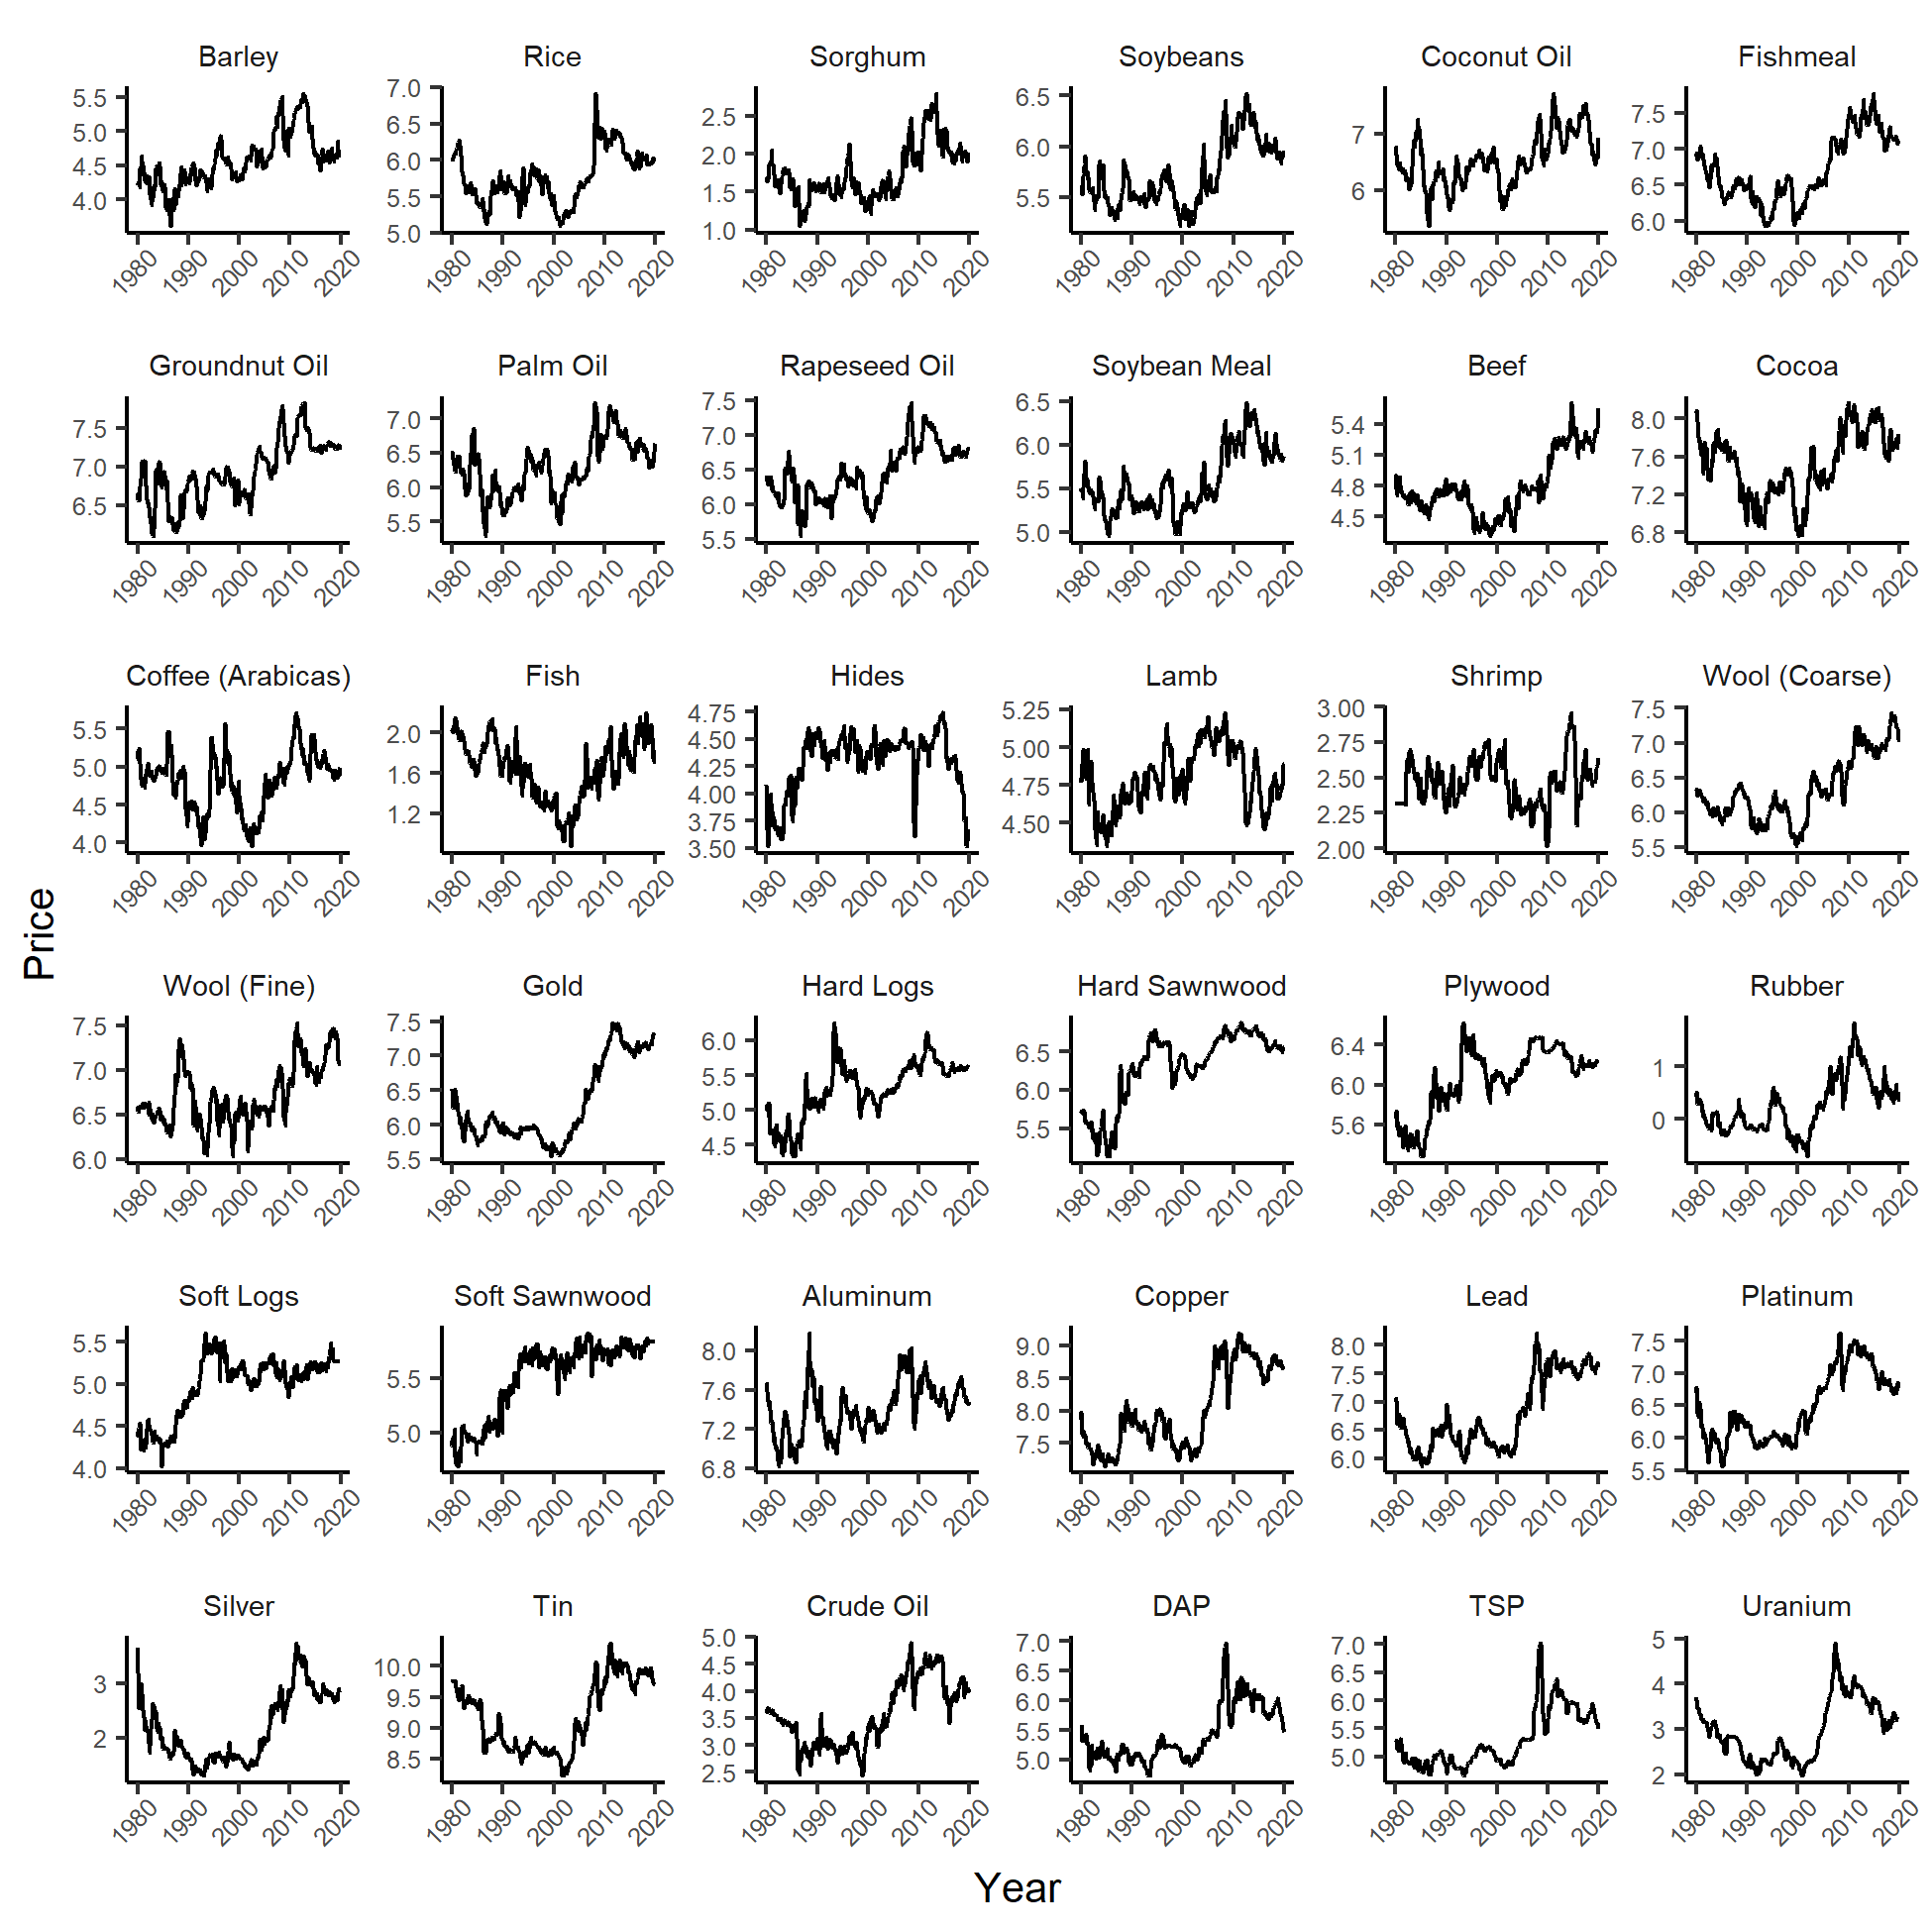
\includegraphics[scale=1]{../Prices}
	\caption{Time Series of the Commodity Prices Used in the Analysis}
	\label{prices}
	\textit{Note}: The price series are log-transformed. Appendix Table~\ref{tab:a1} presents the description, including the units of measurement, of these commodity prices. 
\end{figure}

For each price series, I decided on the order of integration (based on the augmented Dickey--Fuller test), and the autoregressive lag length (based on the Schwartz Information Criterion subject to no remaining residual autocorrelation) using the data ranging the January 1982 -- December 2019 period. That is, the series exclude first 24 months, which were reserved for lag selection and for testing linearity against multistep STAR models. I tested the null hypotheses of linearity against STAR alternatives using lagged dependent variables, up to the selected autoregressive order, as candidate transition variables. This is to decide on a suitable transition variable, as well as the form of a transition function---logistic or exponential---as discussed in the previous section. Using the same order of integration and the autoregressive order, I also tested the null hypotheses of linearity against multistep STAR alternatives to decide on the horizon--specific suitable transition variables and the form of transition functions. The resulting functional forms are then imposed onto the commodity price series in each and every rolling window. That is, in any rolling window, and for a given horizon, forecasts are obtained assuming the same STAR specification. Figure~\ref{tfunc} illustrates the estimated transition functions plotted against to the selected transition variables (denoted by $s_t$, which can be either $y_{t-d}$ or $\Delta y_{t-d+1}$, where $d \in 1,\ldots,p$.) 
\begin{figure}
	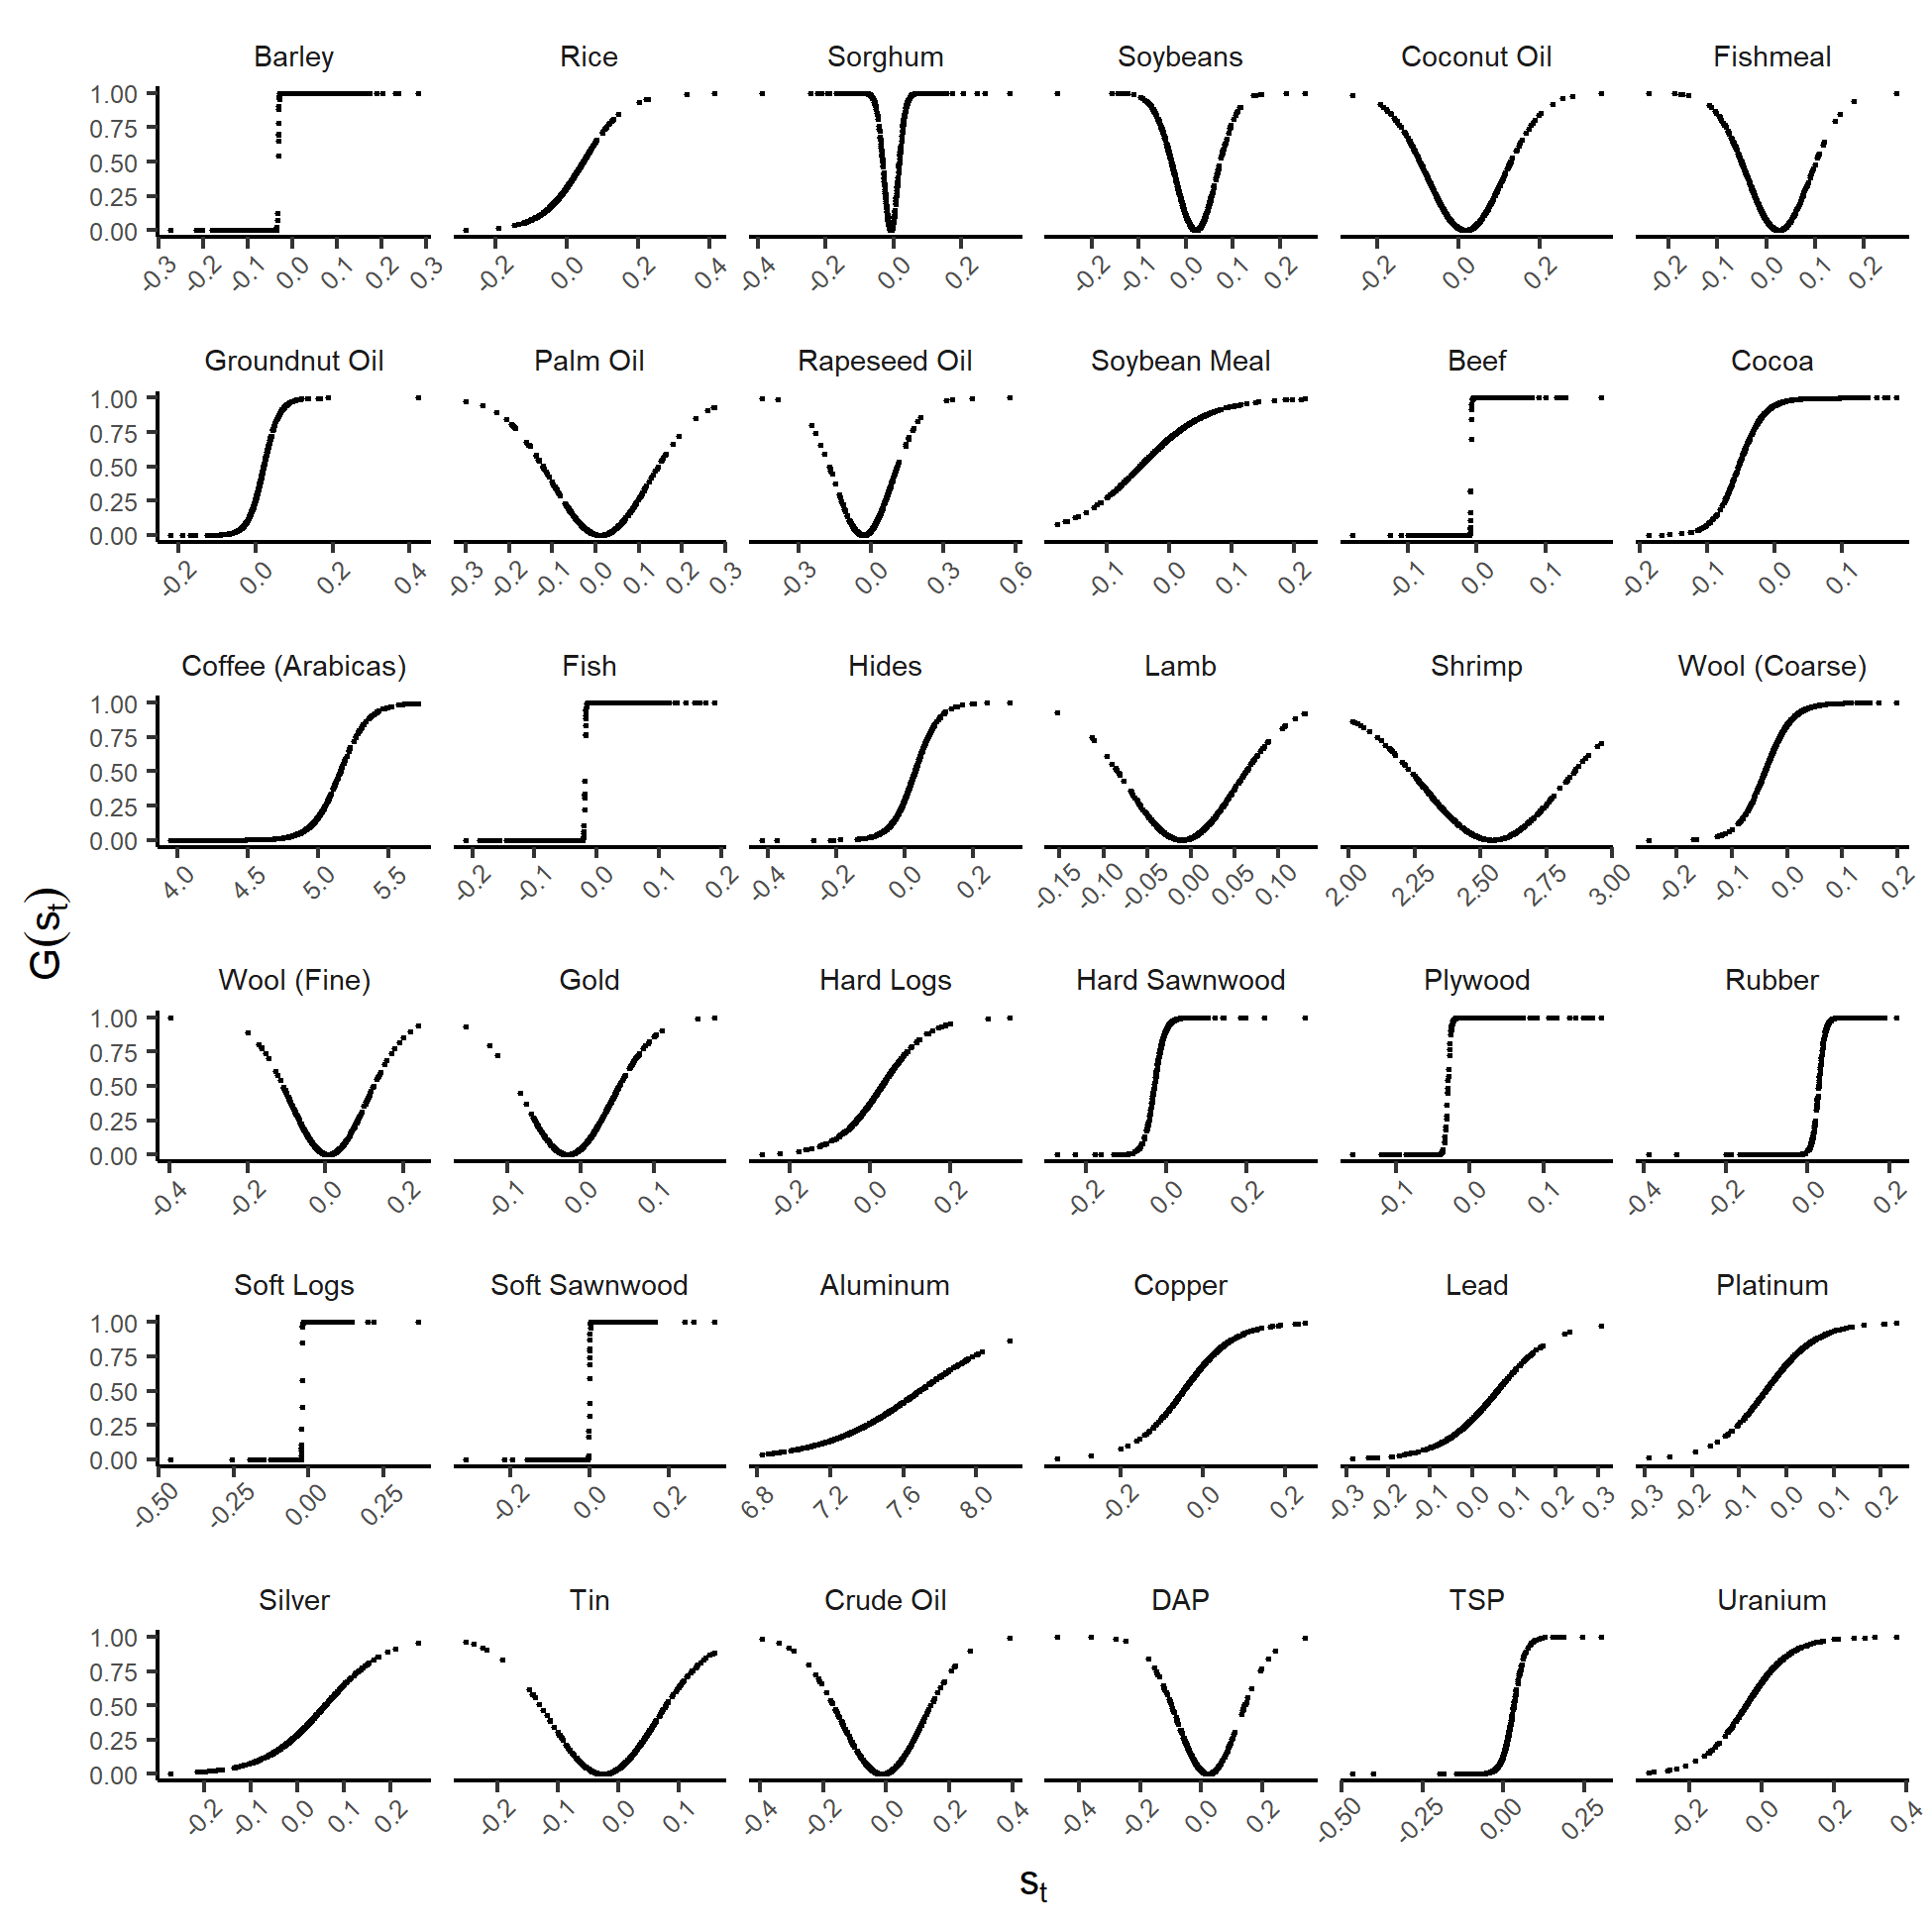
\includegraphics[scale=1]{../Transition_Functions}
	\caption{Estimated Transition Functions Against Selected Transition Variables}
	\label{tfunc}
	\textit{Note}:
\end{figure}

To set up a forecasting routine, I use 80 percent of the price series (360 observations) for model estimation, and the remaining 20 percent of the series (84 observations) for out-of-sample evaluation of one-to-twelve-months-ahead forecasts.\footnote{As a robustness check, I repeated the forecasting exercise for the 75/25 and the 85/15 sample splits. The results of this check are available in the Appendix.} Throughout I use a rolling window approach. Thus, the first estimation window spans the January 1982 -- December 2011 period, yielding forecasts for months of January 2012 through December 2012. The second estimation window spans the February 1982 -- January 2012 period, yielding forecasts for February 2012 through January 2013. All the subsequent estimation windows are rolled in a similar fashion, the very last estimation window yielding forecasts for months of December 2018 through November 2019. 

For each rolling window, I generate iterated multistep forecasts from a one-step STAR model, by iterating forward 5,000 projections, using the bootstrap procedure outlined in the previous section; the horizon-specific averages of these projections form the iterated multistep forecasts. I also generate direct multistep forecasts from horizon-specific STAR models. 

Note that for the I(1) series, I slightly modify equations~\eqref{iteratedar}~and~\eqref{iteratedstar} (for iterated forecasts) and equations~\eqref{directar}~and~\eqref{directstar} (for direct forecasts). In the case of the iterated method, first I obtain the forecast path up to horizon $h$ of the first-differenced series; then I calculate an $h$-step-ahead forecast: $\hat{y}_{T+h}^i = y_{T} + \sum_{j=1}^{h}\Delta\hat{y}_{T+j}^i$, where $\Delta$ is the first-difference operator, and $\Delta\hat{y}_{T+j}^i$, $j=1,\ldots,h$, are obtained iteratively, as described above, using parameter estimates of a regression of $\Delta y_t$ on $\Delta y_{t-1},\ldots,\Delta y_{t-p+1}$. In the case of direct method, an $h$-step-ahead forecast becomes: $\hat{y}_{T+h}^d = y_{T} + \hat{x}_{T+h}$, where the second term is the point forecast of $x_{T+h} = y_{T+h} - y_{T}$, which is obtained by first regressing $x_t$ on $\Delta y_{t-h},\ldots,\Delta y_{t-h-p+2}$, and then applying the parameter estimates of this regression on $\Delta y_{t},\ldots,\Delta y_{t-p+2}$. 

Thus, for each commodity price series, and for each considered horizon, $h=1,\ldots,12$, I generate two sets of forecasts, $\hat{y}_{T+h}^{i,n}$ and $\hat{y}_{T+h}^{d,n}$, from STAR specifications. In addition, I generate two sets of forecasts, $\hat{y}_{T+h}^{i,l}$ and $\hat{y}_{T+h}^{d,l}$, using AR specifications (i.e., the linear counterparts of the previous two forecasts). This yields 84 point forecasts for each horizon, for the out-of-sample period from January 2012 onward.


\section{Forecast Evaluation and Discussion}

I evaluate forecast accuracy under the assumption of a quadratic loss---a widely accepted loss function, particularly as it relates to the implicit criterion for in-sample fitting of the data (i.e., minimizing the sum of squared residuals). In particular, for a given forecast, $\hat{y}_{T+h}$, the out-of-sample forecast error is $e_{T+h} = y_{T+h}-\hat{y}_{T+h}$ (here, and in what follows, I omit the method and model superscripts for ease of notation). The quadratic loss leads to the root mean squared forecast error (RMSFE), given by: $$\text{RMSFE} = \sqrt{\frac{1}{T_2-T_1+1}\sum_{T=T_1}^{T_2}e_{T+h}^2},$$ where $T_1$ denotes the period at which the first forecast is made, and $T_2$ denotes the period at which the last forecast is made. For each commodity price series, and each horizon, I assess the accuracy of forecasts from two competing methods (or models) by comparing the respective RMSFEs. To get further insights for the degree (or, rather, the statistical significance) of the differences in RMSFEs, I perform horizon--specific tests for the equal predictive accuracy as per \cite{diebold1995}, using \cite{harvey1997}--modified test statistics. In addition, as a single measure of multi-horizon accuracy, I apply the average superior predictive ability method of \cite{quaedvlieg2021} for each considered horizon (i.e., for horizons 2 to 12).

To begin, I compare RMSFEs of forecasts from iterated and direct STAR methods. Table~\ref{nlstar} presents the relative RMSFEs, together with the single-horizon and multi-horizon statistical significance identifiers. Overall, the iterated STAR method appears to be more accurate than the direct STAR method in multistep commodity price forecasting (e.g., rice, soybeans, shrimp, and the wood varieties), but there are also instances when the opposite appears to be the case (e.g., groundnut oil, beef, and some metals). Notably, there are instances when one-step-ahead forecasts from STAR models do not outperform a simple random walk specification---a feature that appears to be more common for metals. 
\begin{table}[hbtp]
	\caption{Relative RMSFEs of Iterated STAR vs. Direct STAR Methods}
	\label{nlstar}
	\footnotesize
	\begin{tabular*}{1.0\textwidth}{@{\extracolsep{\linewidth minus\linewidth}}lS[table-format=1.3]S[table-format=1.3]S[table-format=1.3]S[table-format=1.3]S[table-format=1.3]S[table-format=1.3]S[table-format=1.3]S[table-format=1.3]S[table-format=1.3]S[table-format=1.3]S[table-format=1.3]S[table-format=1.3]}
		\toprule
		Commodity & \multicolumn{12}{c}{\textit{horizon}} \\
		&   1	&	2		&	3		&	4		&	5		&	6		&	7		&	8		&	9		&	10		&	11		&	12	\\
		\midrule
		Barley 			& 0.976 & 0.975 & 0.952 & 0.976 & 0.980 & 0.996 & 1.004 & 1.017 & 1.001 & 0.987 & 1.003 & 0.983 \\ 
		Rice 			& 1.023 & 0.996 & 1.015 & 0.965 & 0.971 & 0.949$^*$ & 0.924$^*$ & 0.920 & 0.905$^*$$^{\dagger}$ & 0.901$^{\dagger}$ & 0.917$^{\dagger}$ & 0.949$^{\dagger}$ \\ 
		Sorghum 		& 1.077 & 0.988 & 1.052 & 0.984 & 1.052 & 1.036 & 1.071 & 1.024 & 1.048 & 0.991 & 1.025 & 0.979 \\ 
		Soybeans 		& 1.017 & 0.980 & 0.982$^{\dagger}$ & 0.997 & 1.002 & 0.993 & 0.986 & 0.963 & 0.936$^*$ & 0.946$^{\dagger}$ & 0.939$^{\dagger}$ & 0.929$^{\dagger}$ \\ 
		Coconut Oil 	& 1.022 & 1.007 & 1.009 & 1.037 & 1.055 & 1.051 & 1.029 & 1.006 & 1.001 & 1.010 & 0.997 & 1.000 \\ 
		Fishmeal 		& 0.902$^*$ & 1.013 & 1.015 & 1.002 & 0.999 & 1.009 & 1.011 & 1.005 & 1.019 & 1.008 & 1.015 & 1.012 \\ 
		Groundnut Oil 	& 0.889 & 1.021 & 1.014 & 1.013$^*$ & 1.035$^*$ & 1.032$^{\dagger}$ & 1.053 & 1.041 & 1.037 & 1.035 & 1.035 & 1.043 \\ 
		Palm Oil 		& 0.949$^*$ & 1.039 & 0.996 & 1.021 & 0.978 & 0.979 & 0.991 & 0.976 & 0.959 & 0.959 & 0.956 & 0.950 \\ 
		Rapeseed Oil 	& 1.001 & 1.002 & 1.021 & 0.987 & 0.962 & 0.972 & 0.943 & 0.941$^*$ & 0.933 & 0.918 & 0.901 & 0.896 \\ 
		Soybean Meal 	& 0.910 & 0.965 & 0.991 & 0.954 & 0.963 & 0.955 & 0.967 & 0.972 & 0.978 & 0.982 & 0.977 & 1.026 \\ 
		Beef 			& 0.955 & 0.999 & 1.020 & 1.037 & 1.048 & 1.041 & 1.053 & 1.043 & 1.032 & 1.028 & 1.003 & 1.024$^*$ \\ 
		Cocoa 			& 0.961 & 0.964 & 0.979 & 0.939 & 0.944 & 0.953 & 0.978 & 0.989 & 0.992 & 0.992 & 1.001 & 1.023 \\ 
		Coffee (Arabicas) & 0.935 & 0.997 & 1.007 & 1.004 & 1.005 & 0.977 & 1.022 & 1.064 & 1.026 & 1.086 & 1.131 & 1.124 \\ 
		Fish 			& 1.031 & 0.961 & 0.967 & 0.982 & 0.980 & 0.987 & 0.985 & 0.983 & 0.976 & 0.972 & 0.974 & 0.965 \\ 
		Hides 			& 0.945 & 0.996 & 0.978 & 0.979 & 0.994 & 0.996 & 0.996 & 0.976 & 0.994 & 1.012 & 1.032 & 1.034 \\ 
		Lamb 			& 0.884$^*$ & 1.002 & 0.984 & 0.996 & 0.959 & 0.959 & 0.964 & 0.962 & 0.964 & 0.964 & 0.950 & 0.943 \\ 
		Shrimp 			& 0.769 & 0.930$^*$$^{\dagger}$ & 0.902$^{\dagger}$ & 0.900$^*$$^{\dagger}$ & 0.961$^{\dagger}$ & 0.847$^{\dagger}$ & 0.859 & 0.936 & 0.991 & 1.026 & 0.976 & 0.988 \\ 
		Wool (Coarse) 	& 0.982 & 0.994 & 1.003 & 0.984 & 0.985 & 0.975 & 0.992 & 1.004 & 0.969 & 0.970 & 0.973 & 0.972 \\ 
		Wool (Fine) 	& 0.982 & 0.979 & 0.973$^*$$^{\dagger}$ & 0.979 & 0.987 & 1.004 & 0.981 & 0.984 & 0.963 & 0.941 & 0.940 & 0.969 \\ 
		Gold 			& 0.996 & 0.988 & 0.999 & 0.997 & 0.999 & 0.988 & 0.992 & 0.993 & 0.994 & 0.984 & 0.975 & 0.971 \\ 
		Hard Logs 		& 1.021 & 1.025 & 0.956 & 0.929 & 0.952 & 0.982 & 0.970 & 0.940 & 0.867 & 0.865 & 0.859 & 0.853 \\ 
		Hard Sawnwood 	& 1.108$^*$$^{\dagger}$ & 1.020$^*$$^{\dagger}$ & 0.970 & 0.887$^*$$^{\dagger}$ & 0.937$^*$$^{\dagger}$ & 0.960$^*$$^{\dagger}$ & 0.976$^{\dagger}$ & 0.995$^{\dagger}$ & 0.977$^{\dagger}$ & 1.018 & 0.961 & 1.018 \\ 
		Plywood 		& 0.996 & 0.997 & 0.958$^{\dagger}$ & 0.982$^{\dagger}$ & 0.956 & 0.968 & 0.969 & 0.982 & 0.985 & 0.970$^*$$^{\dagger}$ & 0.941$^*$$^{\dagger}$ & 0.949$^*$$^{\dagger}$ \\ 
		Rubber 			& 1.022 & 1.010 & 1.001 & 1.012 & 1.029 & 1.008 & 1.013 & 1.023 & 1.032 & 1.031 & 1.016 & 1.038 \\ 
		Soft Logs 		& 0.986 & 1.005 & 0.998 & 0.993 & 1.005 & 0.965$^*$ & 1.011 & 0.966 & 0.989 & 0.934$^*$ & 0.955$^*$ & 0.987 \\ 
		Soft Sawnwood 	& 0.986 & 1.010 & 0.993 & 0.995 & 1.024 & 1.014 & 1.007 & 0.993 & 0.955 & 1.008 & 1.000 & 0.982 \\ 
		Aluminum 		& 1.065$^*$ & 1.027 & 1.088 & 1.077$^*$ & 1.021 & 1.045 & 1.065 & 1.037 & 1.083 & 1.049 & 1.044 & 1.086 \\ 
		Copper 			& 0.987 & 0.969$^*$$^{\dagger}$ & 0.978 & 0.977 & 0.965 & 0.964 & 0.968 & 0.955 & 0.948 & 0.966 & 0.964 & 0.958 \\ 
		Lead 			& 1.072 & 1.021$^*$$^{\dagger}$ & 1.014 & 0.991 & 0.984 & 0.977 & 0.999 & 0.983 & 0.995 & 0.991 & 0.986 & 1.002 \\ 
		Platinum 		& 1.017 & 1.018$^*$$^{\dagger}$ & 1.014 & 1.022 & 1.041 & 1.045 & 1.039 & 1.037 & 1.028 & 1.062 & 1.075 & 1.067 \\ 
		Silver 			& 0.991 & 0.981 & 1.007 & 0.992 & 0.976 & 0.971 & 0.932$^*$ & 0.972 & 0.965 & 0.966 & 0.968 & 0.966 \\ 
		Tin 			& 1.017 & 1.009 & 1.032 & 1.057 & 1.048 & 1.030 & 1.039 & 1.056 & 1.023 & 1.034 & 1.056 & 1.073$^*$ \\ 
		Crude Oil 		& 0.944 & 0.989 & 0.994 & 1.023 & 1.011 & 1.016 & 1.002 & 1.001 & 1.008 & 1.005 & 0.997 & 0.985 \\ 
		DAP 			& 0.972 & 0.977 & 0.952 & 1.000 & 1.013 & 1.009 & 1.017 & 1.029 & 1.041 & 1.025 & 1.012 & 1.023 \\ 
		TSP 			& 1.028 & 1.003 & 1.024 & 1.032 & 1.032 & 1.002 & 1.009 & 0.962 & 0.911 & 0.956 & 0.973 & 0.987 \\ 
		Uranium 		& 1.005 & 1.040$^*$$^{\dagger}$ & 1.061$^{\dagger}$ & 1.085 & 1.048 & 1.038 & 1.018 & 0.999 & 0.985 & 0.978 & 0.960 & 0.973 \\ 
		\bottomrule
	\end{tabular*}
	\textit{Note}: The entries for the horizon 1 are the RMSFEs of a STAR model relative to the random walk; the entries for the horizons 2 to 12 are the RMSFEs of the iterated STAR method relative to the direct STAR method; $^{*}$ denotes 5\% statistical significance of the loss differential of the given horizon, and $^{\dagger}$ denotes 5\% statistical significance of the sum of loss differentials up to a given horizon, as per \cite{quaedvlieg2021}; both tests are based on the heteroskedasticity and autocorrelation consistent t distribution of the \cite{harvey1997}--modified \cite{diebold1995} statistic.
\end{table}

Next, I evaluate the forecast accuracy of the iterated STAR method relative to the direct AR method. This is of specific interest to the present study as one of the main arguments for the use of a direct method to generate forecasts is when the one-step model is believed to be misspecified. Table~\ref{niterldir} presents this comparison, as before accompanied by the associated statistical significance tests. One key general take-away from these results is that the iterated STAR method outperforms the direct AR method in forecasting most agricultural commodity prices; however, the direct AR method is preferred to the iterated STAR method in forecasting metal and other non-agricultural commodity prices, even though the STAR-type nonlinearity is the characterizing feature of these price dynamics.
\begin{table}[hbtp]
	\caption{Relative RMSFEs of Iterated STAR vs. Direct AR Methods}
	\label{niterldir}
	\footnotesize
	\begin{tabular*}{1.0\textwidth}{@{\extracolsep{\linewidth minus\linewidth}}lS[table-format=1.3]S[table-format=1.3]S[table-format=1.3]S[table-format=1.3]S[table-format=1.3]S[table-format=1.3]S[table-format=1.3]S[table-format=1.3]S[table-format=1.3]S[table-format=1.3]S[table-format=1.3]S[table-format=1.3]}
	\toprule
		Commodity & \multicolumn{12}{c}{\textit{horizon}} \\
		&	1	&	2	&	3	&	4	&	5	&	6	&	7	&	8	&	9	&	10	&	11	&	12	\\
		\midrule
		Barley 			& 1.003 & 0.985 & 0.979 & 0.989 & 1.002 & 1.009 & 1.019 & 1.018 & 1.008 & 1.005 & 1.003 & 0.997 \\ 
		Rice 			& 1.075$^*$$^{\dagger}$ & 1.036 & 1.019 & 1.010 & 1.001 & 0.983 & 1.001 & 1.005 & 1.009 & 0.998 & 0.994 & 1.007 \\ 
		Sorghum 		& 1.038 & 0.967 & 1.041 & 1.006 & 1.068 & 1.044 & 1.075 & 1.029 & 1.051 & 1.013 & 1.033 & 0.990 \\ 
		Soybeans 		& 1.007 & 0.999 & 0.985 & 0.982 & 0.978 & 0.961 & 0.962 & 0.970 & 0.952 & 0.954 & 0.953 & 0.950 \\ 
		Coconut Oil 	& 1.005 & 1.018 & 1.014 & 1.024 & 1.043 & 1.029 & 1.016 & 1.004 & 0.996 & 1.003 & 0.986 & 0.982 \\ 
		Fishmeal 		& 0.990 & 0.979 & 0.984 & 0.970 & 0.977 & 0.987 & 0.980 & 0.971 & 0.975 & 0.972 & 0.981 & 0.974 \\ 
		Groundnut Oil 	& 1.013 & 1.014 & 1.005 & 0.996 & 1.010 & 1.009 & 0.999 & 1.011 & 1.019 & 1.036 & 1.055 & 1.071 \\ 
		Palm Oil 		& 1.013 & 1.032 & 1.034 & 1.025 & 0.998 & 0.990 & 0.992 & 0.988 & 0.983 & 0.978 & 0.981 & 0.991 \\ 
		Rapeseed Oil 	& 0.985 & 0.999 & 1.016 & 1.004 & 0.985 & 0.978 & 0.992 & 0.972 & 0.971 & 0.959 & 0.948 & 0.951 \\ 
		Soybean Meal 	& 0.997 & 0.986 & 0.981 & 0.983 & 0.987 & 0.989 & 0.995 & 0.998 & 0.995 & 0.998 & 0.997 & 0.997 \\ 
		Beef 			& 1.019 & 1.001 & 1.003 & 1.014 & 1.026 & 1.036 & 1.044 & 1.043 & 1.035$^*$ & 1.032 & 1.029 & 1.033 \\ 
		Cocoa 			& 0.978 & 0.975 & 0.980 & 0.962 & 0.973 & 0.978 & 0.992 & 1.000 & 1.004 & 1.016 & 1.016 & 1.034 \\ 
		Coffee (Arabicas) & 0.988 & 0.981 & 0.983 & 0.978 & 0.972 & 0.962 & 0.955$^*$ & 0.952$^*$ & 0.948$^*$ & 0.937 & 0.924$^*$$^{\dagger}$ & 0.923 \\ 
		Fish 			& 1.017 & 0.993 & 0.996 & 1.012 & 1.011 & 1.016 & 1.012 & 1.011 & 1.015 & 1.008 & 1.016 & 1.012 \\ 
		Hides 			& 1.011 & 1.012 & 1.015 & 1.004 & 1.004 & 0.999 & 0.989 & 0.980 & 0.992 & 1.004 & 1.018 & 1.015 \\ 
		Lamb 			& 0.987 & 0.993 & 0.989 & 0.969$^*$ & 0.957$^*$$^{\dagger}$ & 0.940$^*$$^{\dagger}$ & 0.941$^*$$^{\dagger}$ & 0.942$^{\dagger}$ & 0.943 & 0.953 & 0.964 & 0.960 \\ 
		Shrimp 			& 1.029$^*$$^{\dagger}$ & 1.018 & 1.019 & 1.018 & 1.015 & 1.016 & 1.018 & 1.019 & 1.014 & 1.022 & 1.030 & 1.034 \\ 
		Wool (Coarse) 	& 1.011 & 1.011 & 1.013 & 1.008 & 1.004 & 1.010 & 1.020$^*$ & 1.020 & 1.005 & 1.010 & 1.009 & 1.002 \\ 
		Wool (Fine) 	& 1.021 & 1.025 & 1.037 & 1.035 & 1.055 & 1.070 & 1.060 & 1.045 & 1.011 & 0.988 & 0.983 & 0.992 \\ 
		Gold 			& 0.999 & 0.994 & 1.008 & 0.997 & 0.997 & 0.996 & 0.994 & 0.993 & 0.996 & 0.993 & 0.989 & 0.984 \\ 
		Hard Logs 		& 1.009 & 1.008 & 0.989 & 0.981 & 0.975 & 0.968 & 0.964 & 0.968 & 0.933$^*$ & 0.936 & 0.918 & 0.910 \\ 
		Hard Sawnwood 	& 1.056$^*$$^{\dagger}$ & 1.030 & 1.002 & 0.972 & 0.987 & 0.994 & 0.990 & 0.985 & 0.979 & 0.986 & 0.948 & 0.963 \\ 
		Plywood 		& 0.998 & 0.987 & 0.984 & 0.984 & 0.984 & 0.992 & 0.998 & 0.997 & 0.998 & 0.984 & 0.978 & 0.982 \\ 
		Rubber 			& 1.053$^*$$^{\dagger}$ & 1.037 & 1.017 & 1.026 & 1.038$^*$ & 1.043$^*$$^{\dagger}$ & 1.040$^{\dagger}$ & 1.047$^*$$^{\dagger}$ & 1.050$^*$$^{\dagger}$ & 1.046$^*$$^{\dagger}$ & 1.031$^{\dagger}$ & 1.039$^*$$^{\dagger}$ \\ 
		Soft Logs 		& 1.024$^*$$^{\dagger}$ & 1.023$^*$$^{\dagger}$ & 1.003 & 0.997 & 0.999 & 1.004 & 1.005 & 0.991 & 0.996 & 1.000 & 1.006 & 1.002 \\ 
		Soft Sawnwood 	& 0.988 & 1.005 & 1.010 & 1.033 & 1.032 & 1.028 & 1.022 & 1.020 & 1.012 & 1.044 & 1.023 & 1.011 \\ 
		Aluminum 		& 1.057$^*$$^{\dagger}$ & 1.090$^*$$^{\dagger}$ & 1.111$^*$$^{\dagger}$ & 1.131$^*$$^{\dagger}$ & 1.127$^*$$^{\dagger}$ & 1.126$^*$$^{\dagger}$ & 1.145$^*$$^{\dagger}$ & 1.156$^*$$^{\dagger}$ & 1.156$^*$$^{\dagger}$ & 1.171$^*$$^{\dagger}$ & 1.207$^*$$^{\dagger}$ & 1.192$^*$$^{\dagger}$ \\ 
		Copper 			& 1.005 & 1.000 & 1.007 & 1.016 & 1.016 & 1.009 & 1.006 & 0.988 & 0.996 & 0.987 & 0.981 & 0.995 \\ 
		Lead 			& 1.071$^*$$^{\dagger}$ & 1.048$^*$$^{\dagger}$ & 1.043$^*$$^{\dagger}$ & 1.018$^{\dagger}$ & 1.015 & 1.010 & 1.009 & 1.018 & 1.024 & 1.020 & 1.008 & 1.025 \\ 
		Platinum 		& 1.011 & 1.017 & 1.024 & 1.028 & 1.040$^*$ & 1.046$^*$ & 1.047$^*$$^{\dagger}$ & 1.046$^*$$^{\dagger}$ & 1.042$^*$$^{\dagger}$ & 1.056$^*$$^{\dagger}$ & 1.056$^*$$^{\dagger}$ & 1.048$^*$$^{\dagger}$ \\ 
		Silver 			& 0.998 & 0.993 & 0.993 & 0.993 & 0.985 & 0.984 & 0.980 & 0.999 & 0.975 & 0.984 & 0.983 & 0.991 \\ 
		Tin 			& 1.024 & 1.034 & 1.050 & 1.061 & 1.070 & 1.074 & 1.086 & 1.100 & 1.080 & 1.084 & 1.072 & 1.095$^*$ \\ 
		Crude Oil 		& 0.994 & 1.011 & 1.013 & 1.025 & 1.020 & 1.013 & 1.009 & 0.999 & 1.012 & 1.010 & 0.996 & 0.989 \\ 
		DAP 			& 0.957 & 0.967 & 0.970 & 0.975 & 0.969 & 0.990 & 1.004 & 1.012 & 1.025 & 1.016 & 1.020 & 1.030$^*$ \\ 
		TSP 			& 1.046 & 1.045 & 1.035 & 1.037 & 1.026 & 1.007 & 1.025 & 1.019 & 1.020 & 1.026 & 1.029 & 1.032 \\ 
		Uranium 		& 1.077 & 1.060 & 1.027 & 1.000 & 0.994 & 1.026 & 1.042 & 1.044 & 1.034 & 1.029 & 1.015 & 1.019 \\
		\bottomrule
	\end{tabular*}
	\textit{Note}: The entries are the RMSFEs of the iterated STAR method relative to the direct AR method (for the horizon 1, the entries, by default, are the RMSFEs of a STAR model relative to an AR model); $^{*}$ denotes 5\% statistical significance of the loss differential of the given horizon, and $^{\dagger}$ denotes 5\% statistical significance of the sum of loss differentials up to a given horizon, as per \cite{quaedvlieg2021}; both tests are based on the heteroskedasticity and autocorrelation consistent t distribution of the \cite{harvey1997}--modified \cite{diebold1995} statistic.
\end{table}

At this point, a question is whether the nonlinear modeling facilitates more accurate forecasting of the considered commodity prices. Table~\ref{niterliter} addresses this question by presenting the ratios of RMSFEs from the iterated STAR method relative to the iterated AR method. In some agricultural commodities, specifically soybeans and coffee, there is evidence of improved forecast accuracy, particularly at longer horizons. An improved forecast accuracy, albeit not statistically significant, is also observed in several other agricultural commodities, such as fishmeal, soybean meal, coconut oil, and rapeseed oil. For non-agricultural commodities, there is hardly any evidence that the nonlinear modeling benefits price forecasting; indeed, in most instances, there is strong evidence that AR models outperform STAR models in generating accurate multistep forecasts. This is not an unusual finding, and indeed, it accords with the existing literature; the possible explanations include parameter non-constancy in the time series, as well as misspecification and over-fitting of the nonlinear model \citep{terasvirta2006}.
\begin{table}[hbtp]
	\caption{Relative RMSFEs of Iterated STAR vs. Iterated AR Methods}
	\label{niterliter}
	\footnotesize
	\begin{tabular*}{1.0\textwidth}{@{\extracolsep{\linewidth minus\linewidth}}lS[table-format=1.3]S[table-format=1.3]S[table-format=1.3]S[table-format=1.3]S[table-format=1.3]S[table-format=1.3]S[table-format=1.3]S[table-format=1.3]S[table-format=1.3]S[table-format=1.3]S[table-format=1.3]S[table-format=1.3]}
		\toprule
		Commodity & \multicolumn{12}{c}{\textit{horizon}} \\
						&	1	&	2	&	3	&	4	&	5	&	6	&	7	&	8	&	9	&	10	&	11	&	12	\\
		\midrule
		Barley 			& 1.003 & 0.993 & 0.998 & 1.005 & 1.011 & 1.014 & 1.018 & 1.022 & 1.021 & 1.017 & 1.015 & 1.015 \\ 
		Rice 			& 1.075$^*$$^{\dagger}$ & 1.038 & 1.019 & 1.011 & 1.005 & 1.000 & 1.008 & 1.013 & 1.009 & 1.005 & 1.008 & 1.013 \\ 
		Sorghum 		& 1.038 & 0.965 & 1.025 & 0.990 & 1.035 & 1.003 & 1.043 & 1.008 & 1.041$^*$ & 1.004 & 1.039 & 0.996 \\ 
		Soybeans 		& 1.007 & 1.005 & 0.989 & 0.978 & 0.971 & 0.964 & 0.962$^*$ & 0.968 & 0.958 & 0.952 & 0.947$^*$ & 0.944$^*$$^{\dagger}$ \\ 
		Coconut Oil 	& 1.005 & 1.006 & 0.992 & 0.988 & 0.989 & 0.986 & 0.985 & 0.985 & 0.984 & 0.983 & 0.982 & 0.982 \\ 
		Fishmeal 		& 0.990 & 0.985 & 0.988 & 0.982 & 0.982 & 0.984 & 0.980 & 0.976 & 0.974$^*$ & 0.974 & 0.978 & 0.979 \\ 
		Groundnut Oil 	& 1.013 & 1.014 & 1.006 & 0.998 & 1.002 & 1.010 & 1.017 & 1.025 & 1.041 & 1.055 & 1.061 & 1.063 \\ 
		Palm Oil 		& 1.013 & 1.033 & 1.033 & 1.015 & 1.005 & 1.003 & 1.007 & 1.005 & 1.002 & 1.001 & 0.999 & 1.001 \\ 
		Rapeseed Oil 	& 0.985 & 1.002 & 1.013 & 0.997 & 0.992 & 0.982 & 0.982 & 0.979 & 0.980 & 0.975 & 0.972 & 0.970 \\ 
		Soybean Meal 	& 0.997 & 0.990 & 0.982 & 0.984 & 0.987 & 0.986 & 0.986 & 0.986 & 0.985 & 0.985 & 0.984 & 0.982 \\ 
		Beef 			& 1.019 & 1.001 & 1.004 & 1.005 & 1.011 & 1.018 & 1.024$^*$ & 1.026$^*$ & 1.027$^*$$^{\dagger}$ & 1.028$^*$$^{\dagger}$ & 1.024$^*$$^{\dagger}$ & 1.019$^*$$^{\dagger}$ \\ 
		Cocoa 			& 0.978 & 0.977 & 0.980 & 0.971 & 0.974 & 0.984 & 0.989 & 0.992 & 0.996 & 1.003 & 1.007 & 1.014 \\ 
		Coffee (Arabicas) & 0.988 & 0.985 & 0.979 & 0.974 & 0.966 & 0.959 & 0.952$^*$ & 0.944$^*$ & 0.940$^*$ & 0.936$^*$ & 0.932$^*$$^{\dagger}$ & 0.929$^*$$^{\dagger}$ \\ 
		Fish 			& 1.017 & 0.993 & 0.996 & 1.008 & 1.013 & 1.011 & 1.000 & 0.994 & 0.999 & 1.007 & 1.010 & 1.010 \\ 
		Hides 			& 1.011 & 1.015 & 1.021 & 1.021 & 1.022$^*$ & 1.031$^*$ & 1.031$^*$$^{\dagger}$ & 1.033$^{\dagger}$ & 1.037$^{\dagger}$ & 1.042$^{\dagger}$ & 1.049$^{\dagger}$ & 1.054$^{\dagger}$ \\ 
		Lamb 			& 0.987 & 0.999 & 0.997 & 0.993 & 0.990 & 0.986 & 0.986 & 0.988 & 0.990 & 0.989 & 0.988 & 0.988 \\ 
		Shrimp 			& 1.029$^*$$^{\dagger}$ & 1.026 & 1.032 & 1.036 & 1.036 & 1.035 & 1.035 & 1.036 & 1.038 & 1.041 & 1.040 & 1.036 \\ 
		Wool (Coarse) 	& 1.011 & 1.004 & 1.001 & 0.999 & 0.998 & 0.999 & 0.998 & 0.999 & 1.002 & 1.001 & 0.998 & 1.000 \\ 
		Wool (Fine) 	& 1.021 & 1.029 & 1.043 & 1.045 & 1.046 & 1.048 & 1.041 & 1.031 & 1.014 & 0.997 & 0.992 & 0.992 \\ 
		Gold 			& 0.999 & 0.994 & 1.001 & 0.997 & 0.997 & 0.999 & 1.000 & 1.000 & 0.998 & 0.997 & 0.998 & 0.999 \\ 
		Hard Logs 		& 1.009 & 0.999 & 0.992 & 0.986 & 0.983 & 0.980 & 0.981 & 0.984 & 0.985 & 0.987 & 0.989 & 0.992 \\ 
		Hard Sawnwood 	& 1.056$^*$$^{\dagger}$ & 1.038$^{\dagger}$ & 1.025 & 1.007 & 0.999 & 0.997 & 0.995 & 0.991 & 0.985 & 0.983 & 0.982 & 0.980 \\ 
		Plywood 		& 0.998 & 0.985 & 0.986 & 0.987 & 0.990 & 0.992 & 0.992 & 0.992 & 0.994 & 0.994 & 0.995 & 0.996 \\ 
		Rubber 			& 1.053$^*$$^{\dagger}$ & 1.040$^{\dagger}$ & 1.019 & 1.015 & 1.022 & 1.027 & 1.031 & 1.040$^*$ & 1.045$^*$ & 1.043$^*$ & 1.039$^*$ & 1.040$^*$ \\ 
		Soft Logs 		& 1.024$^*$$^{\dagger}$ & 1.019$^*$$^{\dagger}$ & 1.010$^{\dagger}$ & 0.998 & 0.994 & 0.996 & 0.994 & 0.993 & 0.999 & 0.995 & 0.998 & 1.000 \\ 
		Soft Sawnwood 	& 0.988 & 1.004 & 0.997 & 1.003 & 1.002 & 1.001 & 0.994 & 0.995 & 0.994 & 0.997 & 0.998 & 0.988 \\ 
		Aluminum 		& 1.057$^*$$^{\dagger}$ & 1.098$^*$$^{\dagger}$ & 1.118$^*$$^{\dagger}$ & 1.135$^*$$^{\dagger}$ & 1.129$^*$$^{\dagger}$ & 1.138$^*$$^{\dagger}$ & 1.144$^*$$^{\dagger}$ & 1.136$^*$$^{\dagger}$ & 1.141$^*$$^{\dagger}$ & 1.144$^*$$^{\dagger}$ & 1.156$^*$$^{\dagger}$ & 1.162$^*$$^{\dagger}$ \\ 
		Copper 			& 1.005 & 1.002 & 1.003 & 1.008 & 1.013 & 1.012 & 1.010 & 1.011 & 1.012$^*$ & 1.014$^*$ & 1.014 & 1.011 \\ 
		Lead 			& 1.071$^*$$^{\dagger}$ & 1.046$^*$$^{\dagger}$ & 1.035$^*$$^{\dagger}$ & 1.022$^{\dagger}$ & 1.019$^{\dagger}$ & 1.024$^*$$^{\dagger}$ & 1.024$^{\dagger}$ & 1.020$^{\dagger}$ & 1.015 & 1.018 & 1.016 & 1.021 \\ 
		Platinum 		& 1.011 & 1.018 & 1.025 & 1.032 & 1.041 & 1.043 & 1.041 & 1.041 & 1.047 & 1.050 & 1.054$^*$ & 1.054$^*$ \\ 
		Silver 			& 0.998 & 0.996 & 1.001 & 1.000 & 0.994 & 0.991 & 0.990 & 0.991 & 0.987 & 0.986 & 0.987 & 0.988 \\ 
		Tin 			& 1.024 & 1.034 & 1.045 & 1.051 & 1.054 & 1.064 & 1.076 & 1.083$^*$$^{\dagger}$ & 1.078$^*$$^{\dagger}$ & 1.084$^*$$^{\dagger}$ & 1.080$^*$$^{\dagger}$ & 1.073$^*$$^{\dagger}$ \\ 
		Crude Oil 		& 0.994 & 1.012 & 1.009 & 1.013 & 1.016 & 1.011 & 1.003 & 1.001 & 1.002 & 1.004 & 1.003 & 1.002 \\ 
		DAP 			& 0.957 & 0.962 & 0.963 & 0.962 & 0.972 & 0.983 & 0.988 & 0.986 & 0.985 & 0.988 & 0.993 & 0.997 \\ 
		TSP 			& 1.046 & 1.040 & 1.034 & 1.029 & 1.025 & 1.023 & 1.023 & 1.022 & 1.019 & 1.015 & 1.014 & 1.013 \\ 
		Uranium 		& 1.077 & 1.057 & 1.018 & 0.983 & 0.976 & 1.013 & 1.047 & 1.058 & 1.053 & 1.038 & 1.025 & 1.020 \\ 
		\bottomrule
	\end{tabular*}
	\textit{Note}: The entries are the RMSFEs of the iterated forecasts from a STAR model relative to an AR model; $^{*}$ denotes 5\% statistical significance of the loss differential of the given horizon, and $^{\dagger}$ denotes 5\% statistical significance of the sum of loss differentials up to a given horizon, as per \cite{quaedvlieg2021}; both tests are based on the heteroskedasticity and autocorrelation consistent t distribution of the \cite{harvey1997}--modified \cite{diebold1995} statistic.
\end{table}



\section{Conclusion}

This study empirically investigates the possible advantage of an iterated multistep method over a direct multistep method in forecasting primary commodity prices using smooth transition autoregressive models. From an array of 53 primary commodity prices, the analysis focuses on 18 price series, which present strong evidence of STAR-type nonlinear dynamics. Overall, the findings indicate that while STAR models can well approximate nonlinear dynamics of commodity price series, when it comes to multistep forecasting, the framework doesn't offer an advantage, and indeed, in most instances appears to be an inferior alternative to the basic autoregressive framework. While for select individual commodities a case can be made for either of the considered methods, general recommendation---based on the results of this study---is that linear methods are to be seen as safer approach for their multistep forecasting.


\newpage
\singlespacing
\bibliographystyle{chicago}
\bibliography{mybib}

\newpage
\onehalfspacing
\appendix

\setcounter{table}{0}
\renewcommand{\thetable}{A\arabic{table}}

\setcounter{figure}{0}
\renewcommand{\thefigure}{A\arabic{figure}}

\section{Tables}

\begin{table}[H]
	\caption{The Details of the Commodity Price Series Used in the Analysis}
	\label{tab:a1}
	\small
	\begin{tabular*}{1.0\textwidth}{@{\extracolsep{\linewidth minus\linewidth}}>{\ttfamily}lp{5.75in}}
		\toprule
		Abbrev	&	Description and Origin	\\[2pt]
		\midrule
		ALMN	&	Aluminum, 99.5\% minimum purity, LME spot price, CIF UK ports, \$/mt	\\
		BEEF	&	Beef, Australian and New Zealand 85\% lean fores, CIF U.S. import price, c/lb	\\
%		BNNA	&	Bananas, Central American and Ecuador, FOB U.S. Ports, \$/mt	\\
%		BRLY	&	Barley, Canadian no.1 Western Barley, spot price, \$/mt	\\
		CARB	&	Coffee, Other Mild Arabicas, ICO New York cash price, ex-dock New York, c/lb	\\
		CCOA	&	Cocoa beans, ICO cash price, CIF U.S. and European ports, \$/mt	\\
%		CHIK	&	Poultry (chicken), Whole bird spot price, Ready-to-cook, whole, iced, Georgia docks, US cents/lb	\\
%		CNOL	&	Coconut oil (Philippines/Indonesia), crude, CIF NW Europe beg. 1999; prev. bulk, CIF Rotterdam	\\
		COIL	&	Crude Oil (petroleum), West Texas Intermediate 40 API, Midland Texas, \$/barrel	\\
%		COTN	&	Cotton, Cotton Outlook `A Index', Middling 1-3/32 inch staple, CIF Liverpool, US cents/lb	\\
		CPPR	&	Copper, grade A cathode, LME spot price, CIF European ports, \$/mt	\\
		CRBS	&	Coffee, Robusta, ICO New York cash price, ex-dock New York, c/lb	\\
		DAPP	&	DAP (diammonium phosphate), spot, FOB U.S. Gulf	\\
%		FISH	&	Fish (salmon), Farm Bred Norwegian Salmon, export price, \$ per kilogram	\\
		FSML	&	Fishmeal, Peru Fish meal/pellets 65\% protein, CIF, \$/mt	\\
		GNOL	&	Groundnut oil, U.S. crude, FOB SE beg. 1999; prev. any origin, CIF Rotterdam.	\\
%		GNUT	&	Groundnuts (US), Runners 40/50, CFR NW Europe beg. 1999; prev. (US), shelled basis, CIF Rotterdam	\\
		GOLD	&	Gold (UK), 99.5\% fine, London afternoon fixing, average of daily rates	\\
		HIDE	&	Hides, heavy native steers over 53 pounds, wholesale dealer's price, Chicago FOB Shipping Point, c/lb	\\
%		LAMB	&	Lamb, frozen carcass Smithfield London, US cents/lb	\\
		LEAD	&	Lead, 99.97\% pure, LME spot price, CIF European Ports, \$/mt	\\
		LGHD	&	Hard Logs, Best quality Malaysian meranti, import price Japan, \$/m$^3$	\\
		LGST	&	Soft Logs, Average Export price from the U.S. for Douglas Fir, \$/m$^3$	\\
%		MAZE	&	Maize (corn), U.S. no.2 Yellow, FOB Gulf of Mexico, U.S. price, \$/mt	\\
%		NCKL	&	Nickel, melting grade, LME spot price, CIF European ports, \$/mt	\\
%		ORNG	&	Oranges (Mediterranean exporters) navel, European Union indicative import price, CIF Paris	\\
		OVOL	&	Olive Oil, extra virgin less than 1\% free fatty acid, ex-tanker price U.K., \$/mt	\\
		PLAT	&	Platinum (UK), 99.9\% refined, London afternoon fixing	\\
		PLWD	&	Plywood (Africa and Southeast Asia), Lauan, 3-ply, extra, 91cm$\times$182cm$\times$4mm,  wholesale price, spot Tokyo	\\
		PMOL	&	Palm oil (Malaysia), RBD, CIF Rotterdam beg. Dec 2001; prev. 5\%, CIF NW Europe, bulk, nearest forward	\\
%		PORK	&	Swine (pork), 51-52\% lean Hogs, U.S. price, US cents/lb	\\
		RICE	&	Rice, 5 percent broken milled white rice, Thailand nominal price quote, \$/mt	\\
		RPOL	&	Rapeseed oil, crude, fob Rotterdam, \$/mt	\\
		RUBR	&	Rubber (any origin), Ribbed Smoked Sheet (RSS) no.1, in bales, RTA, spot, New York	\\
%		SBEN	&	Soybeans, U.S. no.2 yellow meal, CIF Rotterdam beg. Dec 2007; prev. U.S. origin, nearest forward.	\\
%		SBML	&	Soybean meal, Brazilian pellets 48\%, CIF Rotterdam beg. 1999; 1990 - 1998 45/46\%, nearest forward; prev. U.S. origin 44\%	\\
		SBOL	&	Soybean oil, Dutch crude degummed, FOB NW Europe beg. 1999; prev. FOB ex-mill Netherlands, nearest forward	\\
%		SILV	&	Silver (UK), 99.9\% refined, London afternoon fixing	\\
		SRGM	&	Sorghum; U.S., Number 2 yellow, fob Gulf of Mexico, c/lb	\\
		SRMP	&	Shrimp (US), brown, shell-on, headless, 26--30 count/lb, wholesale Gulf of Mexico beg. 2004; prev. New York.	\\
%		SUGR	&	Sugar (world), ISA daily price, raw,  FOB and stowed at greater Caribbean ports	\\
		SWHD	&	Hard Sawnwood, Dark Red Meranti, select and better quality, C\&F U.K port, \$/m$^3$	\\
		SWST	&	Soft Sawnwood, average export price of Douglas Fir, U.S. Price, \$/m$^3$	\\
%		TBAC	&	Tobacco (any origin), unmanufactured, general import, CIF, U.S. 	\\
%		TEAM	&	Tea (Mombasa/Nairobi auctions), African origin, all tea, arithmetic average of weekly quotes.	\\
		TINN	&	Tin, standard grade, LME spot price, \$/mt	\\
		TSPP	&	TSP (triple superphosphate), spot, import U.S. Gulf	\\
		URAN	&	Uranium, NUEXCO, Restricted Price, Nuexco exchange spot, \$/lb	\\
%		UREA	&	US Gulf NOLA Urea Granular Spot Price, USD/ST	\\
%		WHET	&	Wheat, no.1 Hard Red Winter, ordinary protein, Kansas City, \$/mt	\\
%		WLCS	&	Wool, coarse, 23 micron, Australian Wool Exchange spot quote, US cents per kilogram	\\
%		WLFN	&	Wool, fine, 19 micron, Australian Wool Exchange spot quote, US cents per kilogram	\\
%		ZINC	&	Zinc, high grade 98\% pure, \$/mt	\\
		\bottomrule
	\end{tabular*}
\end{table}


\begin{table}[hbtp]
	\caption{Linearity Test Results}
	\label{lintest}
	\footnotesize
	\begin{tabular*}{1.0\textwidth}{@{\extracolsep{\linewidth minus\linewidth}}lS[table-format=1.3]S[table-format=1.3]S[table-format=1.3]S[table-format=1.3]S[table-format=1.3]S[table-format=1.3]S[table-format=1.3]S[table-format=1.3]S[table-format=1.3]S[table-format=1.3]S[table-format=1.3]S[table-format=1.3]}
		\toprule
		Commodity & \multicolumn{12}{c}{\textit{horizon}} \\
		&	1	&	2	&	3	&	4	&	5	&	6	&	7	&	8	&	9	&	10	&	11	&	12	\\
		\midrule
		Barley	&	0.005	&	0.053	&	0.070	&	0.160	&	0.311	&	0.613	&	0.776	&	0.616	&	0.453	&	0.415	&	0.545	&	0.863	\\
		Rice	&	0.001$^*$	&	0.001$^*$	&	0.001$^*$	&	0.001	&	0.001$^*$	&	0.001$^*$	&	0.001$^*$	&	0.014	&	0.069	&	0.088	&	0.051	&	0.084	\\
		Sorghum	&	0.001$^*$	&	0.001$^*$	&	0.001$^*$	&	0.001$^*$	&	0.001$^*$	&	0.011	&	0.036	&	0.105	&	0.175	&	0.157	&	0.123	&	0.021	\\
		Soybeans	&	0.001$^*$	&	0.002	&	0.005	&	0.009	&	0.014	&	0.025	&	0.036	&	0.018	&	0.083	&	0.024	&	0.021	&	0.005	\\
		Coconut Oil	&	0.044	&	0.007	&	0.102	&	0.068	&	0.039	&	0.019	&	0.035	&	0.061	&	0.051	&	0.043	&	0.009	&	0.007	\\
		Fishmeal	&	0.003	&	0.003	&	0.001	&	0.001$^*$	&	0.001	&	0.002	&	0.001	&	0.002	&	0.005	&	0.026	&	0.047	&	0.026	\\
		Groundnut Oil	&	0.001$^*$	&	0.001$^*$	&	0.001$^*$	&	0.001$^*$	&	0.001$^*$	&	0.003	&	0.003	&	0.013	&	0.024	&	0.092	&	0.137	&	0.086	\\
		Palm Oil	&	0.001$^*$	&	0.006	&	0.033	&	0.142	&	0.273	&	0.275	&	0.610	&	0.568	&	0.423	&	0.697	&	0.685	&	0.665	\\
		Rapeseed Oil	&	0.001$^*$	&	0.001$^*$	&	0.007	&	0.001	&	0.001$^*$	&	0.005	&	0.099	&	0.089	&	0.370	&	0.374	&	0.254	&	0.242	\\
		Soybean Meal	&	0.017	&	0.025	&	0.190	&	0.065	&	0.040	&	0.160	&	0.312	&	0.292	&	0.411	&	0.184	&	0.085	&	0.043	\\
		Beef	&	0.001$^*$	&	0.021	&	0.008	&	0.004	&	0.009	&	0.076	&	0.184	&	0.060	&	0.058	&	0.104	&	0.116	&	0.051	\\
		Cocoa	&	0.017	&	0.034	&	0.178	&	0.534	&	0.549	&	0.611	&	0.569	&	0.578	&	0.352	&	0.182	&	0.219	&	0.378	\\
		Coffee (Arabicas)	&	0.009	&	0.007	&	0.004	&	0.006	&	0.006	&	0.009	&	0.012	&	0.006	&	0.003	&	0.001$^*$	&	0.001$^*$	&	0.001$^*$	\\
		Fish	&	0.030	&	0.035	&	0.168	&	0.141	&	0.231	&	0.418	&	0.448	&	0.487	&	0.306	&	0.274	&	0.222	&	0.240	\\
		Hides	&	0.001$^*$	&	0.001$^*$	&	0.001$^*$	&	0.002	&	0.002	&	0.001	&	0.001	&	0.002	&	0.001$^*$	&	0.001$^*$	&	0.001$^*$	&	0.001$^*$	\\
		Lamb	&	0.002	&	0.001$^*$	&	0.002	&	0.016	&	0.002	&	0.001	&	0.007	&	0.034	&	0.060	&	0.046	&	0.042	&	0.028	\\
		Shrimp	&	0.001$^*$	&	0.001$^*$	&	0.001$^*$	&	0.001$^*$	&	0.001$^*$	&	0.001$^*$	&	0.001$^*$	&	0.001$^*$	&	0.001$^*$	&	0.001$^*$	&	0.001$^*$	&	0.001$^*$	\\
		Wool (Coarse)	&	0.022	&	0.597	&	0.788	&	0.737	&	0.381	&	0.119	&	0.082	&	0.071	&	0.033	&	0.014	&	0.007	&	0.004	\\
		Wool (Fine)	&	0.033	&	0.028	&	0.008	&	0.008	&	0.008	&	0.011	&	0.013	&	0.054	&	0.054	&	0.029	&	0.023	&	0.014	\\
		Gold	&	0.003	&	0.038	&	0.360	&	0.939	&	0.842	&	0.395	&	0.549	&	0.518	&	0.266	&	0.178	&	0.490	&	0.172	\\
		Hard Logs	&	0.001$^*$	&	0.001$^*$	&	0.001$^*$	&	0.001$^*$	&	0.001$^*$	&	0.001	&	0.001$^*$	&	0.001$^*$	&	0.001$^*$	&	0.003	&	0.033	&	0.065	\\
		Hard Sawnwood	&	0.001$^*$	&	0.010	&	0.001$^*$	&	0.001$^*$	&	0.001$^*$	&	0.001$^*$	&	0.001	&	0.002	&	0.001$^*$	&	0.001$^*$	&	0.001$^*$	&	0.001$^*$	\\
		Plywood	&	0.001	&	0.024	&	0.033	&	0.015	&	0.087	&	0.147	&	0.322	&	0.270	&	0.282	&	0.371	&	0.415	&	0.357	\\
		Rubber	&	0.001$^*$	&	0.001$^*$	&	0.032	&	0.009	&	0.033	&	0.021	&	0.003	&	0.001$^*$	&	0.001$^*$	&	0.001$^*$	&	0.001$^*$	&	0.001$^*$	\\
		Soft Logs	&	0.001$^*$	&	0.001$^*$	&	0.009	&	0.011	&	0.026	&	0.011	&	0.036	&	0.049	&	0.022	&	0.061	&	0.178	&	0.175	\\
		Soft Sawnwood	&	0.001$^*$	&	0.001$^*$	&	0.001$^*$	&	0.008	&	0.005	&	0.042	&	0.069	&	0.009	&	0.128	&	0.027	&	0.126	&	0.228	\\
		Aluminum	&	0.001$^*$	&	0.004	&	0.001	&	0.001$^*$	&	0.001$^*$	&	0.001$^*$	&	0.001$^*$	&	0.001$^*$	&	0.001$^*$	&	0.001$^*$	&	0.001$^*$	&	0.001$^*$	\\
		Copper	&	0.001$^*$	&	0.007	&	0.002	&	0.001$^*$	&	0.001$^*$	&	0.001$^*$	&	0.001$^*$	&	0.001$^*$	&	0.001$^*$	&	0.001$^*$	&	0.001$^*$	&	0.001$^*$	\\
		Lead	&	0.001$^*$	&	0.008	&	0.010	&	0.019	&	0.015	&	0.044	&	0.059	&	0.012	&	0.004	&	0.002	&	0.001	&	0.007	\\
		Platinum	&	0.002	&	0.003	&	0.007	&	0.034	&	0.010	&	0.002	&	0.001$^*$	&	0.001$^*$	&	0.001$^*$	&	0.001$^*$	&	0.004	&	0.004	\\
		Silver	&	0.010	&	0.040	&	0.147	&	0.076	&	0.016	&	0.007	&	0.008	&	0.056	&	0.321	&	0.186	&	0.119	&	0.060	\\
		Tin	&	0.001$^*$	&	0.058	&	0.079	&	0.040	&	0.094	&	0.234	&	0.366	&	0.178	&	0.185	&	0.254	&	0.251	&	0.261	\\
		Crude Oil	&	0.032	&	0.031	&	0.179	&	0.047	&	0.049	&	0.031	&	0.012	&	0.008	&	0.002	&	0.003	&	0.006	&	0.014	\\
		DAP	&	0.001$^*$	&	0.001$^*$	&	0.001	&	0.004	&	0.001$^*$	&	0.001$^*$	&	0.001$^*$	&	0.009	&	0.028	&	0.099	&	0.064	&	0.061	\\
		TSP	&	0.001	&	0.118	&	0.356	&	0.298	&	0.339	&	0.318	&	0.265	&	0.079	&	0.002	&	0.001$^*$	&	0.001$^*$	&	0.001$^*$	\\
		Uranium	&	0.001$^*$	&	0.001$^*$	&	0.001$^*$	&	0.001$^*$	&	0.001$^*$	&	0.001$^*$	&	0.001	&	0.002	&	0.001	&	0.002	&	0.001$^*$	&	0.001$^*$	\\
		\bottomrule
	\end{tabular*}
	\textit{Note}: The entries are probability values of \cite{terasvirta1994}'s linearity test and its \cite{enders2015} multistep variant. $^*$ denotes probability values that are smaller than those presented in the table.
\end{table}


\begin{table}[hbtp]
	\caption{Relative RMSFEs of Iterated STAR vs. Direct STAR Methods (75/25 split)}
	\label{nlstar75}
	\footnotesize
	\begin{tabular*}{1.0\textwidth}{@{\extracolsep{\linewidth minus\linewidth}}lS[table-format=1.3]S[table-format=1.3]S[table-format=1.3]S[table-format=1.3]S[table-format=1.3]S[table-format=1.3]S[table-format=1.3]S[table-format=1.3]S[table-format=1.3]S[table-format=1.3]S[table-format=1.3]S[table-format=1.3]}
		\toprule
		Commodity & \multicolumn{12}{c}{\textit{horizon}} \\
		&   1	&	2		&	3		&	4		&	5		&	6		&	7		&	8		&	9		&	10		&	11		&	12	\\
		\midrule
		Barley & 0.978 & 0.978 & 0.933 & 0.969 & 0.968 & 0.985 & 0.993 & 1.012 & 0.986 & 0.980 & 0.999 & 0.984 \\ 
		Rice & 0.991 & 1.034 & 1.015 & 0.966 & 0.955 & 0.943 & 0.917 & 0.908 & 0.903 & 0.890 & 0.912 & 0.950 \\ 
		Sorghum & 1.071 & 0.996 & 1.041 & 0.988 & 1.026 & 0.999 & 1.025 & 1.010 & 1.036 & 1.003 & 1.005 & 0.980 \\ 
		Soybeans & 1.002 & 0.995 & 0.987 & 1.022 & 1.026 & 1.021 & 0.991 & 1.006 & 0.988 & 0.987 & 0.986 & 1.005 \\ 
		Coconut Oil & 0.982 & 1.000 & 1.019 & 1.026 & 1.048 & 1.047 & 1.030 & 1.022 & 1.027 & 1.013 & 1.018 & 1.017 \\ 
		Fishmeal & 0.907 & 1.010 & 1.009 & 1.001 & 0.998 & 0.998 & 0.995 & 1.002 & 1.012 & 1.004 & 1.011 & 0.995 \\ 
		Groundnut Oil & 0.837 & 1.029 & 1.028 & 1.021 & 1.025 & 1.026 & 1.020 & 0.995 & 0.995 & 0.985 & 0.952 & 0.958 \\ 
		Palm Oil & 0.937 & 0.988 & 1.024 & 1.048 & 1.049 & 1.031 & 1.039 & 1.024 & 1.019 & 0.994 & 1.015 & 1.001 \\ 
		Rapeseed Oil & 0.970 & 1.003 & 1.036 & 0.991 & 0.985 & 1.002 & 0.996 & 1.003 & 0.976 & 0.986 & 0.978 & 0.982 \\ 
		Soybean Meal & 0.919 & 0.983 & 0.977 & 0.968 & 0.962 & 0.961 & 0.962 & 0.968 & 0.986 & 0.970 & 0.975 & 1.014 \\ 
		Beef & 0.969 & 1.012 & 1.040 & 1.047 & 1.054 & 1.035 & 1.031 & 1.018 & 1.011 & 1.003 & 0.993 & 0.986 \\ 
		Cocoa & 0.954 & 0.958 & 0.978 & 0.944 & 0.959 & 0.953 & 0.971 & 0.976 & 0.986 & 0.986 & 1.000 & 1.008 \\ 
		Coffee (Arabicas) & 1.061 & 1.073 & 1.071 & 1.066 & 1.059 & 0.956 & 0.968 & 0.922 & 0.915 & 0.899 & 0.878 & 0.812 \\ 
		Fish & 1.010 & 0.970 & 0.956 & 0.951 & 0.967 & 0.953 & 0.954 & 0.955 & 0.952 & 0.968 & 0.970 & 0.958 \\ 
		Hides & 0.957 & 0.985 & 0.963 & 0.976 & 0.987 & 1.006 & 1.013 & 0.979 & 0.994 & 1.012 & 1.031 & 1.044 \\ 
		Lamb & 0.924 & 1.013 & 0.991 & 1.005 & 0.967 & 0.965 & 0.957 & 0.952 & 0.959 & 0.975 & 0.959 & 0.970 \\ 
		Shrimp & 0.812 & 0.967 & 0.928 & 0.909 & 0.969 & 0.884 & 0.874 & 0.992 & 0.976 & 1.013 & 0.999 & 1.002 \\ 
		Wool (Coarse) & 0.968 & 0.987 & 0.978 & 0.967 & 0.971 & 0.973 & 0.978 & 0.972 & 0.968 & 0.977 & 0.973 & 0.977 \\ 
		Wool (Fine) & 0.946 & 0.982 & 0.967 & 1.002 & 0.997 & 0.972 & 0.970 & 0.972 & 0.957 & 0.941 & 0.945 & 0.954 \\ 
		Gold & 0.976 & 0.990 & 0.983 & 0.990 & 1.005 & 0.998 & 1.000 & 0.999 & 1.002 & 0.999 & 1.003 & 1.002 \\ 
		Hard Logs & 0.914 & 1.012 & 1.000 & 0.966 & 0.990 & 1.015 & 0.959 & 0.992 & 0.960 & 0.951 & 0.951 & 0.948 \\ 
		Hard Sawnwood & 1.065 & 1.014 & 0.954 & 0.944 & 0.969 & 0.970 & 1.018 & 1.019 & 0.993 & 1.004 & 0.992 & 1.009 \\ 
		Plywood & 1.010 & 0.995 & 0.965 & 0.955 & 0.958 & 0.974 & 0.973 & 0.991 & 0.996 & 1.008 & 0.975 & 0.979 \\ 
		Rubber & 1.010 & 1.014 & 1.017 & 1.015 & 1.029 & 1.012 & 1.006 & 1.017 & 1.012 & 1.012 & 1.014 & 1.056 \\ 
		Soft Logs & 0.985 & 0.994 & 0.989 & 0.982 & 0.978 & 0.977 & 1.013 & 0.957 & 0.997 & 0.958 & 0.972 & 0.975 \\ 
		Soft Sawnwood & 0.951 & 1.014 & 1.000 & 0.994 & 1.021 & 1.020 & 1.012 & 1.009 & 0.966 & 1.005 & 1.024 & 0.968 \\ 
		Aluminum & 1.009 & 0.982 & 0.898 & 0.918 & 0.887 & 0.910 & 0.905 & 0.915 & 0.925 & 0.912 & 0.943 & 0.919 \\ 
		Copper & 0.988 & 0.984 & 0.999 & 1.000 & 0.982 & 0.976 & 0.982 & 0.982 & 0.968 & 0.980 & 0.969 & 0.965 \\ 
		Lead & 1.057 & 1.007 & 0.993 & 0.988 & 0.985 & 0.971 & 0.993 & 0.977 & 0.979 & 0.996 & 0.994 & 1.006 \\ 
		Platinum & 1.008 & 1.009 & 0.987 & 1.000 & 1.013 & 1.019 & 1.004 & 1.010 & 1.014 & 1.023 & 1.042 & 1.035 \\ 
		Silver & 0.996 & 0.991 & 1.006 & 1.007 & 0.997 & 0.962 & 0.962 & 0.976 & 0.970 & 0.978 & 0.975 & 0.973 \\ 
		Tin & 0.989 & 1.003 & 1.014 & 1.015 & 0.995 & 0.995 & 0.971 & 0.971 & 0.966 & 0.989 & 0.967 & 0.968 \\ 
		Crude Oil & 0.962 & 0.987 & 0.976 & 0.998 & 0.999 & 1.003 & 0.987 & 0.990 & 1.002 & 1.000 & 1.002 & 0.987 \\ 
		DAP & 1.077 & 0.973 & 0.953 & 1.008 & 0.977 & 0.981 & 0.969 & 0.966 & 0.905 & 0.963 & 0.961 & 0.981 \\ 
		TSP & 1.022 & 1.001 & 1.008 & 1.025 & 1.021 & 0.978 & 0.959 & 0.951 & 0.869 & 0.869 & 0.897 & 0.918 \\ 
		Uranium & 0.982 & 1.044 & 1.056 & 1.047 & 1.034 & 1.022 & 1.029 & 1.013 & 1.014 & 0.995 & 0.989 & 1.001 \\
		\bottomrule
	\end{tabular*}
	\textit{Note}: The entries for the horizon 1 are the RMSFEs of a STAR model relative to the random walk model; the entries for the horizons 2 to 12 are the RMSFEs of the iterated STAR method relative to the direct STAR method; $^{*}$ denotes 5\% statistical significance of the loss differential of the given horizon, and $^{\dagger}$ denotes 5\% statistical significance of the sum of loss differentials up to a given horizon, as per \cite{quaedvlieg2021}; both tests are based on the heteroskedasticity and autocorrelation consistent t distribution of the \cite{harvey1997}--modified \cite{diebold1995} statistic.
\end{table}


\begin{table}[hbtp]
	\caption{Relative RMSFEs of Iterated STAR vs. Direct AR Methods (75/25 split)}
	\label{niterldir75}
	\footnotesize
	\begin{tabular*}{1.0\textwidth}{@{\extracolsep{\linewidth minus\linewidth}}lS[table-format=1.3]S[table-format=1.3]S[table-format=1.3]S[table-format=1.3]S[table-format=1.3]S[table-format=1.3]S[table-format=1.3]S[table-format=1.3]S[table-format=1.3]S[table-format=1.3]S[table-format=1.3]S[table-format=1.3]}
		\toprule
		Commodity & \multicolumn{12}{c}{\textit{horizon}} \\
		&	1	&	2	&	3	&	4	&	5	&	6	&	7	&	8	&	9	&	10	&	11	&	12	\\
		\midrule
		Barley & 0.992 & 0.970 & 0.972 & 0.981 & 0.998 & 1.006 & 1.004 & 1.012 & 1.001 & 0.997 & 1.001 & 1.002 \\ 
		Rice & 1.054 & 1.040 & 1.023 & 1.016 & 1.013 & 1.008 & 1.006 & 1.003 & 1.011 & 0.995 & 0.997 & 1.009 \\ 
		Sorghum & 1.033 & 0.976 & 1.026 & 1.001 & 1.039 & 1.018 & 1.051 & 1.006 & 1.030 & 1.003 & 1.009 & 0.996 \\ 
		Soybeans & 1.007 & 0.999 & 0.990 & 0.989 & 0.991 & 0.990 & 0.982 & 0.997 & 1.001 & 0.999 & 0.995 & 1.008 \\ 
		Coconut Oil & 0.990 & 1.011 & 1.019 & 1.016 & 1.020 & 1.006 & 1.003 & 0.999 & 1.007 & 0.990 & 0.987 & 0.985 \\ 
		Fishmeal & 0.987 & 0.978 & 0.981 & 0.973 & 0.974 & 0.979 & 0.972 & 0.967 & 0.974 & 0.974 & 0.980 & 0.976 \\ 
		Groundnut Oil & 0.989 & 1.013 & 1.008 & 1.006 & 1.019 & 1.018 & 1.020 & 0.997 & 1.008 & 1.014 & 0.990 & 1.004 \\ 
		Palm Oil & 1.001 & 1.004 & 1.027 & 1.039 & 1.050 & 1.035 & 1.040 & 1.021 & 1.028 & 1.015 & 1.015 & 1.024 \\ 
		Rapeseed Oil & 0.939 & 0.975 & 0.973 & 0.969 & 0.976 & 0.979 & 0.996 & 0.995 & 0.985 & 0.990 & 0.989 & 0.999 \\ 
		Soybean Meal & 1.012 & 0.998 & 0.993 & 0.996 & 0.995 & 1.000 & 0.991 & 0.994 & 0.997 & 0.987 & 0.996 & 1.002 \\ 
		Beef & 1.036 & 1.025 & 1.028 & 1.029 & 1.036 & 1.043 & 1.036 & 1.025 & 1.020 & 1.019 & 1.012 & 1.003 \\ 
		Cocoa & 0.974 & 0.967 & 0.974 & 0.965 & 0.966 & 0.980 & 0.989 & 0.986 & 1.000 & 1.007 & 1.007 & 1.013 \\ 
		Coffee (Arabicas) & 1.095 & 1.122 & 1.145 & 1.151 & 1.145 & 1.142 & 1.124 & 1.118 & 1.109 & 1.096 & 1.076 & 1.049 \\ 
		Fish & 1.020 & 0.991 & 0.980 & 0.994 & 0.986 & 0.991 & 0.988 & 0.987 & 0.986 & 0.990 & 0.994 & 0.996 \\ 
		Hides & 1.009 & 0.999 & 1.001 & 0.991 & 0.990 & 0.999 & 0.998 & 0.988 & 0.993 & 1.006 & 1.021 & 1.027 \\ 
		Lamb & 1.019 & 1.013 & 1.001 & 0.981 & 0.973 & 0.952 & 0.944 & 0.943 & 0.951 & 0.961 & 0.963 & 0.974 \\ 
		Shrimp & 1.056 & 1.047 & 1.040 & 1.019 & 0.999 & 0.997 & 0.999 & 1.005 & 1.006 & 1.008 & 1.012 & 1.006 \\ 
		Wool (Coarse) & 1.018 & 1.012 & 1.016 & 1.019 & 1.018 & 1.011 & 1.012 & 1.004 & 1.004 & 1.010 & 1.002 & 1.005 \\ 
		Wool (Fine) & 1.008 & 0.999 & 1.004 & 1.010 & 1.009 & 1.013 & 1.007 & 1.008 & 0.994 & 0.983 & 0.984 & 0.989 \\ 
		Gold & 0.987 & 0.983 & 0.994 & 0.992 & 0.998 & 1.001 & 1.001 & 1.001 & 1.000 & 0.997 & 1.003 & 1.010 \\ 
		Hard Logs & 1.027 & 1.015 & 1.011 & 1.001 & 1.002 & 1.003 & 1.007 & 1.007 & 1.005 & 0.997 & 0.995 & 0.993 \\ 
		Hard Sawnwood & 1.055 & 1.033 & 1.014 & 1.006 & 1.001 & 1.012 & 1.004 & 0.995 & 0.972 & 0.972 & 0.955 & 0.955 \\ 
		Plywood & 1.011 & 0.996 & 0.984 & 0.979 & 0.975 & 0.985 & 0.990 & 0.997 & 0.997 & 1.016 & 0.996 & 0.993 \\ 
		Rubber & 1.047 & 1.033 & 1.013 & 1.012 & 1.030 & 1.040 & 1.040 & 1.040 & 1.033 & 1.028 & 1.028 & 1.043 \\ 
		Soft Logs & 1.003 & 1.008 & 0.994 & 0.993 & 0.990 & 0.998 & 0.997 & 0.991 & 0.990 & 1.010 & 1.007 & 1.016 \\ 
		Soft Sawnwood & 0.969 & 1.000 & 1.014 & 1.035 & 1.037 & 1.032 & 1.028 & 1.026 & 1.002 & 1.035 & 1.030 & 0.993 \\ 
		Aluminum & 1.010 & 0.994 & 0.983 & 0.978 & 0.959 & 0.960 & 0.946 & 0.953 & 0.938 & 0.936 & 0.955 & 0.967 \\ 
		Copper & 0.999 & 1.015 & 1.020 & 1.017 & 1.014 & 1.004 & 1.006 & 0.998 & 0.991 & 0.994 & 0.991 & 1.002 \\ 
		Lead & 1.054 & 1.035 & 1.009 & 1.009 & 0.993 & 0.986 & 0.991 & 1.000 & 0.993 & 1.019 & 1.018 & 1.037 \\ 
		Platinum & 0.992 & 1.002 & 1.017 & 1.018 & 1.025 & 1.035 & 1.027 & 1.024 & 1.028 & 1.024 & 1.033 & 1.021 \\ 
		Silver & 1.009 & 0.999 & 1.015 & 1.017 & 1.005 & 0.995 & 0.990 & 0.993 & 0.983 & 0.987 & 0.983 & 0.975 \\ 
		Tin & 0.986 & 1.003 & 1.023 & 1.038 & 1.049 & 1.047 & 1.048 & 1.040 & 1.042 & 1.042 & 1.045 & 1.051 \\ 
		Crude Oil & 0.994 & 1.002 & 1.007 & 1.020 & 1.016 & 1.012 & 1.003 & 1.003 & 1.012 & 1.007 & 1.006 & 0.991 \\ 
		DAP & 1.019 & 1.017 & 0.998 & 1.009 & 0.987 & 0.990 & 1.004 & 1.010 & 1.005 & 1.004 & 0.991 & 1.001 \\ 
		TSP & 1.020 & 1.015 & 1.007 & 1.019 & 1.008 & 0.992 & 0.987 & 0.993 & 1.002 & 0.993 & 0.989 & 0.980 \\ 
		Uranium & 1.043 & 1.055 & 1.018 & 0.993 & 1.006 & 1.039 & 1.074 & 1.083 & 1.090 & 1.075 & 1.072 & 1.074 \\
		\bottomrule
	\end{tabular*}
	\textit{Note}: The entries are the RMSFEs of the iterated STAR method relative to the direct AR method (for the horizon 1, the entries, by default, are the RMSFEs of a STAR model relative to an AR model); $^{*}$ denotes 5\% statistical significance of the loss differential of the given horizon, and $^{\dagger}$ denotes 5\% statistical significance of the sum of loss differentials up to a given horizon, as per \cite{quaedvlieg2021}; both tests are based on the heteroskedasticity and autocorrelation consistent t distribution of the \cite{harvey1997}--modified \cite{diebold1995} statistic.
\end{table}


\begin{table}[hbtp]
	\caption{Relative RMSFEs of Iterated STAR vs. Iterated AR Methods (75/25 split)}
	\label{niterliter75}
	\footnotesize
	\begin{tabular*}{1.0\textwidth}{@{\extracolsep{\linewidth minus\linewidth}}lS[table-format=1.3]S[table-format=1.3]S[table-format=1.3]S[table-format=1.3]S[table-format=1.3]S[table-format=1.3]S[table-format=1.3]S[table-format=1.3]S[table-format=1.3]S[table-format=1.3]S[table-format=1.3]S[table-format=1.3]}
		\toprule
		Commodity & \multicolumn{12}{c}{\textit{horizon}} \\
		&	1	&	2	&	3	&	4	&	5	&	6	&	7	&	8	&	9	&	10	&	11	&	12	\\
		\midrule
		Barley & 0.992 & 0.977 & 0.990 & 1.002 & 1.003 & 1.006 & 1.011 & 1.014 & 1.013 & 1.010 & 1.009 & 1.009 \\ 
		Rice & 1.054 & 1.031 & 1.017 & 1.006 & 0.998 & 0.989 & 0.989 & 0.992 & 0.992 & 0.994 & 0.998 & 1.001 \\ 
		Sorghum & 1.033 & 0.979 & 1.021 & 0.994 & 1.031 & 1.007 & 1.039 & 1.009 & 1.035 & 1.007 & 1.035 & 1.003 \\ 
		Soybeans & 1.007 & 1.003 & 0.992 & 0.987 & 0.986 & 0.987 & 0.985 & 0.988 & 0.983 & 0.982 & 0.979 & 0.973 \\ 
		Coconut Oil & 0.990 & 0.999 & 0.995 & 0.987 & 0.986 & 0.980 & 0.981 & 0.983 & 0.982 & 0.982 & 0.979 & 0.979 \\ 
		Fishmeal & 0.987 & 0.983 & 0.984 & 0.980 & 0.979 & 0.980 & 0.976 & 0.974 & 0.973 & 0.974 & 0.978 & 0.978 \\ 
		Groundnut Oil & 0.989 & 1.009 & 1.013 & 1.012 & 1.014 & 1.016 & 1.008 & 0.995 & 0.989 & 0.986 & 0.981 & 0.978 \\ 
		Palm Oil & 1.001 & 1.006 & 1.021 & 1.032 & 1.042 & 1.039 & 1.037 & 1.033 & 1.032 & 1.029 & 1.026 & 1.023 \\ 
		Rapeseed Oil & 0.939 & 0.967 & 0.978 & 0.975 & 0.979 & 0.983 & 0.988 & 0.990 & 0.990 & 0.990 & 0.990 & 0.990 \\ 
		Soybean Meal & 1.012 & 1.008 & 0.999 & 0.998 & 0.996 & 0.991 & 0.988 & 0.988 & 0.987 & 0.987 & 0.986 & 0.985 \\ 
		Beef & 1.036 & 1.030 & 1.030 & 1.023 & 1.024 & 1.024 & 1.024 & 1.017 & 1.011 & 1.010 & 1.007 & 1.003 \\ 
		Cocoa & 0.974 & 0.966 & 0.973 & 0.974 & 0.977 & 0.982 & 0.984 & 0.987 & 0.994 & 1.002 & 1.006 & 1.010 \\ 
		Coffee (Arabicas) & 1.095 & 1.123 & 1.139 & 1.148 & 1.152 & 1.148 & 1.134 & 1.120 & 1.098 & 1.080 & 1.062 & 1.046 \\ 
		Fish & 1.020 & 0.991 & 0.984 & 0.987 & 0.988 & 0.988 & 0.982 & 0.979 & 0.984 & 0.990 & 0.992 & 0.993 \\ 
		Hides & 1.009 & 1.006 & 1.009 & 1.008 & 1.013 & 1.027 & 1.032 & 1.038 & 1.045 & 1.053 & 1.060 & 1.067 \\ 
		Lamb & 1.019 & 1.016 & 1.007 & 1.002 & 0.998 & 0.992 & 0.991 & 0.993 & 0.993 & 0.993 & 0.992 & 0.992 \\ 
		Shrimp & 1.056 & 1.048 & 1.042 & 1.027 & 1.017 & 1.014 & 1.019 & 1.026 & 1.029 & 1.026 & 1.016 & 1.005 \\ 
		Wool (Coarse) & 1.018 & 1.013 & 1.014 & 1.016 & 1.015 & 1.009 & 1.005 & 1.005 & 1.007 & 1.008 & 1.005 & 1.005 \\ 
		Wool (Fine) & 1.008 & 0.999 & 1.007 & 1.012 & 1.012 & 1.011 & 1.006 & 1.001 & 0.994 & 0.990 & 0.990 & 0.992 \\ 
		Gold & 0.987 & 0.984 & 0.997 & 0.993 & 0.995 & 0.998 & 0.999 & 1.000 & 0.999 & 0.998 & 0.999 & 1.001 \\ 
		Hard Logs & 1.027 & 1.018 & 1.011 & 1.004 & 1.003 & 1.004 & 1.005 & 1.003 & 1.001 & 1.001 & 1.000 & 1.000 \\ 
		Hard Sawnwood & 1.055 & 1.036 & 1.033 & 1.018 & 1.014 & 1.011 & 1.004 & 1.000 & 0.994 & 0.993 & 0.992 & 0.990 \\ 
		Plywood & 1.011 & 0.994 & 0.996 & 0.992 & 0.993 & 0.997 & 1.000 & 1.000 & 1.001 & 1.002 & 1.005 & 1.006 \\ 
		Rubber & 1.047 & 1.032 & 1.017 & 1.012 & 1.016 & 1.024 & 1.031 & 1.038 & 1.038 & 1.036 & 1.034 & 1.041 \\ 
		Soft Logs & 1.003 & 1.006 & 1.000 & 0.991 & 0.992 & 0.998 & 0.996 & 0.999 & 1.004 & 0.999 & 1.001 & 1.004 \\ 
		Soft Sawnwood & 0.969 & 1.000 & 1.002 & 1.010 & 1.010 & 1.006 & 1.000 & 1.000 & 0.993 & 0.997 & 1.000 & 0.990 \\ 
		Aluminum & 1.010 & 1.004 & 0.992 & 0.983 & 0.974 & 0.973 & 0.966 & 0.961 & 0.962 & 0.967 & 0.976 & 0.984 \\ 
		Copper & 0.999 & 1.009 & 1.012 & 1.015 & 1.014 & 1.012 & 1.009 & 1.008 & 1.007 & 1.007 & 1.007 & 1.005 \\ 
		Lead & 1.054 & 1.038 & 1.012 & 1.008 & 1.003 & 1.001 & 1.010 & 1.010 & 1.012 & 1.019 & 1.017 & 1.023 \\ 
		Platinum & 0.992 & 1.000 & 1.014 & 1.020 & 1.026 & 1.030 & 1.030 & 1.029 & 1.035 & 1.041 & 1.045 & 1.046 \\ 
		Silver & 1.009 & 1.000 & 1.007 & 1.013 & 1.006 & 0.994 & 0.990 & 0.991 & 0.992 & 0.991 & 0.990 & 0.988 \\ 
		Tin & 0.986 & 1.003 & 1.018 & 1.038 & 1.045 & 1.056 & 1.059 & 1.051 & 1.046 & 1.043 & 1.043 & 1.039 \\ 
		Crude Oil & 0.994 & 1.001 & 1.001 & 1.009 & 1.010 & 1.006 & 1.000 & 1.000 & 1.003 & 1.005 & 1.005 & 1.005 \\ 
		DAP & 1.019 & 1.016 & 1.003 & 1.001 & 1.002 & 1.004 & 1.002 & 1.001 & 0.999 & 0.999 & 1.002 & 1.002 \\ 
		TSP & 1.020 & 1.013 & 1.008 & 1.010 & 1.006 & 1.005 & 1.004 & 1.004 & 1.001 & 0.996 & 0.994 & 0.991 \\ 
		Uranium & 1.043 & 1.053 & 1.016 & 0.995 & 1.007 & 1.041 & 1.079 & 1.093 & 1.093 & 1.085 & 1.078 & 1.075 \\ 
		\bottomrule
	\end{tabular*}
	\textit{Note}: The entries are the RMSFEs of the iterated forecasts from a STAR model relative to an AR model; $^{*}$ denotes 5\% statistical significance of the loss differential of the given horizon, and $^{\dagger}$ denotes 5\% statistical significance of the sum of loss differentials up to a given horizon, as per \cite{quaedvlieg2021}; both tests are based on the heteroskedasticity and autocorrelation consistent t distribution of the \cite{harvey1997}--modified \cite{diebold1995} statistic.
\end{table}


\begin{table}[hbtp]
	\caption{Relative RMSFEs of Iterated STAR vs. Direct STAR Methods (85/15 split)}
	\label{nlstar85}
	\footnotesize
	\begin{tabular*}{1.0\textwidth}{@{\extracolsep{\linewidth minus\linewidth}}lS[table-format=1.3]S[table-format=1.3]S[table-format=1.3]S[table-format=1.3]S[table-format=1.3]S[table-format=1.3]S[table-format=1.3]S[table-format=1.3]S[table-format=1.3]S[table-format=1.3]S[table-format=1.3]S[table-format=1.3]}
		\toprule
		Commodity & \multicolumn{12}{c}{\textit{horizon}} \\
		&   1	&	2		&	3		&	4		&	5		&	6		&	7		&	8		&	9		&	10		&	11		&	12	\\
		\midrule
		Barley & 0.998 & 0.973 & 0.969 & 0.975 & 0.990 & 1.026 & 1.007 & 1.054 & 1.018 & 1.025 & 1.032 & 0.979 \\ 
		Rice & 1.054 & 1.026 & 1.055 & 0.990 & 0.988 & 0.977 & 0.969 & 0.941 & 0.868 & 0.923 & 0.944 & 0.954 \\ 
		Sorghum & 0.991 & 1.008 & 1.025 & 1.006 & 1.045 & 1.053 & 1.061 & 1.070 & 1.053 & 1.047 & 1.041 & 1.068 \\ 
		Soybeans & 1.037 & 0.989 & 0.999 & 0.994 & 0.992 & 1.000 & 0.991 & 1.001 & 0.983 & 0.969 & 0.976 & 0.966 \\ 
		Coconut Oil & 0.996 & 1.019 & 1.000 & 1.030 & 1.028 & 1.038 & 1.022 & 1.021 & 1.036 & 1.043 & 1.043 & 1.064 \\ 
		Fishmeal & 0.873 & 1.018 & 1.024 & 1.005 & 1.016 & 1.021 & 1.030 & 1.029 & 1.026 & 1.021 & 1.016 & 1.001 \\ 
		Groundnut Oil & 0.917 & 0.995 & 1.008 & 1.034 & 1.033 & 1.034 & 1.109 & 1.059 & 1.083 & 1.112 & 1.144 & 1.140 \\ 
		Palm Oil & 0.929 & 1.029 & 0.955 & 0.957 & 0.968 & 0.945 & 0.954 & 0.958 & 0.955 & 1.034 & 0.971 & 1.009 \\ 
		Rapeseed Oil & 0.997 & 0.963 & 1.015 & 1.001 & 0.996 & 1.007 & 0.994 & 0.990 & 1.017 & 0.980 & 0.982 & 0.998 \\ 
		Soybean Meal & 0.891 & 0.959 & 0.964 & 0.909 & 0.931 & 0.924 & 0.937 & 0.942 & 0.966 & 0.954 & 0.974 & 1.002 \\ 
		Beef & 0.958 & 1.002 & 1.032 & 1.049 & 1.052 & 1.038 & 1.051 & 1.045 & 1.026 & 1.015 & 0.992 & 1.034 \\ 
		Cocoa & 0.942 & 0.961 & 0.981 & 0.940 & 0.931 & 0.954 & 0.970 & 0.992 & 0.969 & 0.969 & 0.985 & 0.981 \\ 
		Coffee (Arabicas) & 0.958 & 1.007 & 1.004 & 1.008 & 1.003 & 0.929 & 0.961 & 0.960 & 0.977 & 1.024 & 1.056 & 1.104 \\ 
		Fish & 1.004 & 0.984 & 0.943 & 0.956 & 0.935 & 0.947 & 0.954 & 0.944 & 0.925 & 0.913 & 0.910 & 0.907 \\ 
		Hides & 0.900 & 0.976 & 0.966 & 0.972 & 0.980 & 1.001 & 1.002 & 0.979 & 1.000 & 1.027 & 1.042 & 1.060 \\ 
		Lamb & 0.922 & 1.002 & 0.995 & 1.001 & 0.980 & 0.992 & 0.986 & 0.961 & 0.974 & 0.996 & 0.966 & 0.979 \\ 
		Shrimp & 0.778 & 0.935 & 0.910 & 0.919 & 1.008 & 0.875 & 0.904 & 0.992 & 1.048 & 1.125 & 1.051 & 1.054 \\ 
		Wool (Coarse) & 0.959 & 0.976 & 0.981 & 0.980 & 0.989 & 0.990 & 0.996 & 0.979 & 0.982 & 0.970 & 0.989 & 0.979 \\ 
		Wool (Fine) & 1.025 & 0.983 & 0.977 & 0.942 & 0.918 & 0.931 & 0.894 & 0.905 & 0.915 & 0.918 & 0.927 & 0.947 \\ 
		Gold & 0.993 & 0.996 & 1.014 & 1.012 & 0.986 & 0.982 & 0.977 & 0.967 & 0.954 & 0.940 & 0.926 & 0.925 \\ 
		Hard Logs & 1.010 & 1.003 & 0.946 & 0.985 & 0.993 & 1.027 & 1.017 & 0.954 & 0.904 & 0.910 & 0.920 & 0.913 \\ 
		Hard Sawnwood & 1.103 & 1.011 & 0.972 & 0.900 & 0.903 & 0.913 & 0.920 & 0.925 & 0.940 & 0.952 & 0.937 & 0.962 \\ 
		Plywood & 0.963 & 1.000 & 0.964 & 0.998 & 0.971 & 0.982 & 0.970 & 1.002 & 0.980 & 0.981 & 0.943 & 0.946 \\ 
		Rubber & 0.996 & 0.996 & 0.990 & 0.991 & 1.014 & 0.982 & 0.978 & 1.000 & 1.005 & 0.996 & 1.001 & 1.029 \\ 
		Soft Logs & 1.014 & 0.996 & 0.990 & 0.981 & 0.997 & 0.974 & 1.004 & 0.988 & 1.007 & 0.969 & 0.980 & 1.001 \\ 
		Soft Sawnwood & 0.957 & 1.011 & 1.001 & 0.984 & 0.992 & 0.997 & 0.998 & 1.010 & 1.005 & 1.019 & 1.022 & 0.987 \\ 
		Aluminum & 1.018 & 1.011 & 1.048 & 1.022 & 1.123 & 1.079 & 1.035 & 1.006 & 1.072 & 1.093 & 1.061 & 0.996 \\ 
		Copper & 0.975 & 0.966 & 0.977 & 0.994 & 0.970 & 0.961 & 0.964 & 0.958 & 0.942 & 0.952 & 0.963 & 0.953 \\ 
		Lead & 1.022 & 1.007 & 1.001 & 0.983 & 0.981 & 0.982 & 1.023 & 1.001 & 1.035 & 1.015 & 1.014 & 1.029 \\ 
		Platinum & 1.014 & 1.020 & 1.030 & 1.054 & 1.078 & 1.062 & 1.044 & 1.035 & 1.029 & 1.043 & 1.055 & 1.056 \\ 
		Silver & 1.040 & 0.995 & 1.035 & 1.013 & 1.017 & 1.000 & 0.995 & 0.990 & 0.982 & 0.994 & 0.991 & 0.996 \\ 
		Tin & 1.003 & 1.011 & 1.034 & 1.046 & 1.028 & 1.011 & 1.017 & 1.022 & 1.023 & 1.039 & 1.050 & 1.071 \\ 
		Crude Oil & 0.940 & 0.996 & 1.004 & 1.029 & 1.011 & 1.014 & 0.987 & 1.003 & 1.006 & 1.005 & 0.999 & 0.981 \\ 
		DAP & 0.890 & 0.999 & 0.962 & 1.029 & 1.006 & 1.011 & 0.988 & 0.999 & 1.018 & 0.985 & 0.997 & 0.980 \\ 
		TSP & 1.004 & 1.015 & 1.002 & 1.001 & 0.997 & 0.966 & 0.963 & 1.003 & 0.939 & 0.935 & 0.951 & 1.005 \\ 
		Uranium & 1.023 & 1.033 & 1.060 & 1.082 & 1.043 & 1.038 & 1.026 & 1.026 & 1.025 & 1.023 & 0.999 & 0.996 \\ 
		\bottomrule
	\end{tabular*}
	\textit{Note}: The entries for the horizon 1 are the RMSFEs of a STAR model relative to the random walk model; the entries for the horizons 2 to 12 are the RMSFEs of the iterated STAR method relative to the direct STAR method; $^{*}$ denotes 5\% statistical significance of the loss differential of the given horizon, and $^{\dagger}$ denotes 5\% statistical significance of the sum of loss differentials up to a given horizon, as per \cite{quaedvlieg2021}; both tests are based on the heteroskedasticity and autocorrelation consistent t distribution of the \cite{harvey1997}--modified \cite{diebold1995} statistic.
\end{table}


\begin{table}[hbtp]
	\caption{Relative RMSFEs of Iterated STAR vs. Direct AR Methods (85/15 split)}
	\label{niterldir85}
	\footnotesize
	\begin{tabular*}{1.0\textwidth}{@{\extracolsep{\linewidth minus\linewidth}}lS[table-format=1.3]S[table-format=1.3]S[table-format=1.3]S[table-format=1.3]S[table-format=1.3]S[table-format=1.3]S[table-format=1.3]S[table-format=1.3]S[table-format=1.3]S[table-format=1.3]S[table-format=1.3]S[table-format=1.3]}
		\toprule
		Commodity & \multicolumn{12}{c}{\textit{horizon}} \\
		&	1	&	2	&	3	&	4	&	5	&	6	&	7	&	8	&	9	&	10	&	11	&	12	\\
		\midrule
		Barley & 1.011 & 0.999 & 0.996 & 1.006 & 1.001 & 1.016 & 1.024 & 1.030 & 1.028 & 1.031 & 1.018 & 1.010 \\ 
		Rice & 1.083 & 1.048 & 1.036 & 1.017 & 1.037 & 1.050 & 1.084 & 1.108 & 1.059 & 1.035 & 1.041 & 1.045 \\ 
		Sorghum & 0.968 & 0.983 & 1.015 & 1.045 & 1.064 & 1.079 & 1.094 & 1.092 & 1.070 & 1.096 & 1.086 & 1.086 \\ 
		Soybeans & 1.008 & 1.014 & 1.001 & 1.005 & 0.992 & 0.995 & 0.985 & 1.004 & 1.003 & 0.987 & 0.984 & 0.988 \\ 
		Coconut Oil & 0.969 & 0.990 & 0.999 & 1.011 & 1.019 & 1.014 & 1.009 & 1.010 & 1.018 & 1.022 & 1.015 & 1.027 \\ 
		Fishmeal & 0.963 & 0.978 & 0.999 & 0.983 & 0.988 & 0.991 & 0.995 & 0.982 & 0.982 & 0.987 & 0.984 & 0.971 \\ 
		Groundnut Oil & 1.034 & 1.041 & 1.052 & 1.039 & 1.046 & 1.049 & 1.051 & 1.031 & 1.036 & 1.079 & 1.179 & 1.182 \\ 
		Palm Oil & 0.996 & 0.998 & 0.994 & 0.964 & 0.955 & 0.943 & 0.960 & 0.964 & 0.966 & 0.994 & 0.991 & 1.035 \\ 
		Rapeseed Oil & 0.956 & 0.986 & 1.009 & 0.997 & 1.019 & 1.019 & 1.013 & 1.001 & 1.011 & 1.003 & 1.015 & 1.002 \\ 
		Soybean Meal & 0.985 & 0.974 & 0.964 & 0.967 & 0.972 & 0.977 & 0.986 & 0.988 & 0.983 & 0.981 & 0.991 & 0.987 \\ 
		Beef & 1.028 & 1.009 & 1.019 & 1.029 & 1.032 & 1.036 & 1.043 & 1.037 & 1.048 & 1.050 & 1.053 & 1.052 \\ 
		Cocoa & 0.964 & 0.970 & 0.975 & 0.959 & 0.959 & 0.977 & 0.993 & 0.990 & 0.992 & 1.002 & 0.999 & 1.004 \\ 
		Coffee (Arabicas) & 1.004 & 0.993 & 0.987 & 0.985 & 0.973 & 0.963 & 0.930 & 0.921 & 0.935 & 0.920 & 0.890 & 0.880 \\ 
		Fish & 1.001 & 0.976 & 0.965 & 0.980 & 0.977 & 0.989 & 0.994 & 0.989 & 0.993 & 0.988 & 0.982 & 0.975 \\ 
		Hides & 0.969 & 0.979 & 0.996 & 0.989 & 0.985 & 0.989 & 0.985 & 0.975 & 0.987 & 1.006 & 1.019 & 1.024 \\ 
		Lamb & 0.991 & 0.986 & 0.980 & 0.971 & 0.959 & 0.950 & 0.945 & 0.955 & 0.948 & 0.975 & 0.974 & 0.976 \\ 
		Shrimp & 1.049 & 1.047 & 1.054 & 1.067 & 1.076 & 1.092 & 1.100 & 1.098 & 1.088 & 1.096 & 1.098 & 1.110 \\ 
		Wool (Coarse) & 0.992 & 0.989 & 0.993 & 0.994 & 0.988 & 0.998 & 1.000 & 0.987 & 0.999 & 1.004 & 1.004 & 0.997 \\ 
		Wool (Fine) & 1.035 & 1.049 & 1.059 & 1.045 & 1.035 & 1.017 & 0.988 & 0.986 & 0.976 & 0.966 & 0.968 & 0.977 \\ 
		Gold & 1.007 & 0.991 & 0.994 & 0.991 & 0.989 & 0.988 & 0.980 & 0.975 & 0.968 & 0.957 & 0.958 & 0.965 \\ 
		Hard Logs & 1.005 & 1.006 & 0.995 & 0.999 & 0.997 & 0.997 & 1.000 & 0.980 & 0.962 & 0.968 & 0.984 & 0.978 \\ 
		Hard Sawnwood & 1.058 & 1.022 & 0.987 & 0.973 & 0.969 & 0.960 & 0.941 & 0.934 & 0.933 & 0.925 & 0.915 & 0.894 \\ 
		Plywood & 1.002 & 0.990 & 0.986 & 0.999 & 0.993 & 1.000 & 0.999 & 1.008 & 0.992 & 0.996 & 0.990 & 0.985 \\ 
		Rubber & 1.042 & 1.006 & 1.004 & 1.003 & 1.015 & 1.018 & 1.012 & 1.027 & 1.026 & 1.020 & 1.027 & 1.037 \\ 
		Soft Logs & 1.008 & 1.017 & 1.010 & 1.000 & 0.992 & 1.002 & 1.007 & 0.998 & 1.006 & 1.008 & 1.019 & 1.017 \\ 
		Soft Sawnwood & 0.990 & 1.002 & 0.985 & 0.991 & 0.986 & 1.011 & 1.008 & 1.027 & 1.025 & 1.021 & 1.018 & 0.984 \\ 
		Aluminum & 1.024 & 1.031 & 1.054 & 1.081 & 1.107 & 1.109 & 1.129 & 1.151 & 1.164 & 1.188 & 1.187 & 1.216 \\ 
		Copper & 1.003 & 0.999 & 1.002 & 1.015 & 1.003 & 0.995 & 0.995 & 0.984 & 0.984 & 0.975 & 0.989 & 0.992 \\ 
		Lead & 1.037 & 1.030 & 1.020 & 1.006 & 1.013 & 1.004 & 1.020 & 1.014 & 1.037 & 1.018 & 1.019 & 1.036 \\ 
		Platinum & 1.012 & 1.025 & 1.044 & 1.048 & 1.051 & 1.048 & 1.038 & 1.040 & 1.033 & 1.031 & 1.038 & 1.035 \\ 
		Silver & 1.013 & 1.021 & 1.021 & 1.007 & 1.008 & 1.006 & 1.012 & 1.011 & 1.003 & 1.000 & 1.002 & 1.017 \\ 
		Tin & 1.043 & 1.037 & 1.053 & 1.057 & 1.055 & 1.045 & 1.029 & 1.032 & 1.036 & 1.051 & 1.052 & 1.072 \\ 
		Crude Oil & 0.988 & 1.017 & 1.015 & 1.023 & 1.024 & 1.011 & 0.997 & 1.003 & 1.008 & 1.009 & 1.002 & 0.986 \\ 
		DAP & 0.963 & 0.970 & 0.985 & 0.988 & 0.981 & 1.010 & 0.994 & 0.998 & 1.016 & 0.988 & 1.007 & 0.988 \\ 
		TSP & 1.040 & 1.022 & 1.016 & 1.016 & 1.006 & 1.007 & 1.000 & 1.020 & 1.032 & 1.020 & 1.033 & 1.030 \\ 
		Uranium & 1.048 & 1.057 & 1.026 & 0.996 & 0.993 & 1.035 & 1.068 & 1.065 & 1.076 & 1.071 & 1.056 & 1.046 \\
		\bottomrule
	\end{tabular*}
	\textit{Note}: The entries are the RMSFEs of the iterated STAR method relative to the direct AR method (for the horizon 1, the entries, by default, are the RMSFEs of a STAR model relative to an AR model); $^{*}$ denotes 5\% statistical significance of the loss differential of the given horizon, and $^{\dagger}$ denotes 5\% statistical significance of the sum of loss differentials up to a given horizon, as per \cite{quaedvlieg2021}; both tests are based on the heteroskedasticity and autocorrelation consistent t distribution of the \cite{harvey1997}--modified \cite{diebold1995} statistic.
\end{table}


\begin{table}[hbtp]
	\caption{Relative RMSFEs of Iterated STAR vs. Iterated AR Methods (85/15 split)}
	\label{niterliter85}
	\footnotesize
	\begin{tabular*}{1.0\textwidth}{@{\extracolsep{\linewidth minus\linewidth}}lS[table-format=1.3]S[table-format=1.3]S[table-format=1.3]S[table-format=1.3]S[table-format=1.3]S[table-format=1.3]S[table-format=1.3]S[table-format=1.3]S[table-format=1.3]S[table-format=1.3]S[table-format=1.3]S[table-format=1.3]}
		\toprule
		Commodity & \multicolumn{12}{c}{\textit{horizon}} \\
		&	1	&	2	&	3	&	4	&	5	&	6	&	7	&	8	&	9	&	10	&	11	&	12	\\
		\midrule
		Barley & 1.011 & 0.997 & 0.998 & 1.004 & 1.010 & 1.015 & 1.021 & 1.027 & 1.026 & 1.022 & 1.024 & 1.024 \\ 
		Rice & 1.083 & 1.044 & 1.032 & 1.022 & 1.017 & 1.008 & 1.007 & 1.007 & 0.994 & 0.981 & 0.985 & 0.997 \\ 
		Sorghum & 0.968 & 0.981 & 1.001 & 1.011 & 1.028 & 1.037 & 1.047 & 1.048 & 1.052 & 1.056 & 1.061 & 1.062 \\ 
		Soybeans & 1.008 & 1.012 & 1.001 & 1.001 & 0.998 & 0.994 & 0.994 & 0.993 & 0.993 & 0.986 & 0.979 & 0.979 \\ 
		Coconut Oil & 0.969 & 0.982 & 0.983 & 0.985 & 0.987 & 0.987 & 0.988 & 0.988 & 0.988 & 0.988 & 0.987 & 0.987 \\ 
		Fishmeal & 0.963 & 0.983 & 1.000 & 0.995 & 0.992 & 0.993 & 0.989 & 0.984 & 0.982 & 0.982 & 0.984 & 0.983 \\ 
		Groundnut Oil & 1.034 & 1.036 & 1.037 & 1.029 & 1.038 & 1.056 & 1.074 & 1.085 & 1.095 & 1.107 & 1.107 & 1.084 \\ 
		Palm Oil & 0.996 & 1.003 & 0.987 & 0.955 & 0.940 & 0.945 & 0.957 & 0.960 & 0.963 & 0.974 & 0.983 & 0.989 \\ 
		Rapeseed Oil & 0.956 & 0.975 & 1.000 & 0.996 & 1.012 & 1.004 & 1.007 & 1.001 & 1.003 & 0.997 & 0.987 & 0.981 \\ 
		Soybean Meal & 0.985 & 0.979 & 0.971 & 0.972 & 0.977 & 0.979 & 0.979 & 0.980 & 0.981 & 0.980 & 0.980 & 0.980 \\ 
		Beef & 1.028 & 1.018 & 1.019 & 1.019 & 1.022 & 1.025 & 1.028 & 1.032 & 1.036 & 1.042 & 1.043 & 1.038 \\ 
		Cocoa & 0.964 & 0.970 & 0.972 & 0.966 & 0.970 & 0.980 & 0.987 & 0.993 & 0.998 & 1.004 & 1.009 & 1.014 \\ 
		Coffee (Arabicas) & 1.004 & 0.995 & 0.985 & 0.978 & 0.970 & 0.955 & 0.941 & 0.930 & 0.921 & 0.909 & 0.889 & 0.881 \\ 
		Fish & 1.001 & 0.972 & 0.967 & 0.978 & 0.982 & 0.987 & 0.980 & 0.975 & 0.979 & 0.986 & 0.983 & 0.983 \\ 
		Hides & 0.969 & 0.993 & 1.007 & 1.013 & 1.018 & 1.026 & 1.030 & 1.033 & 1.038 & 1.044 & 1.051 & 1.057 \\ 
		Lamb & 0.991 & 0.984 & 0.982 & 0.979 & 0.974 & 0.967 & 0.967 & 0.971 & 0.974 & 0.974 & 0.972 & 0.974 \\ 
		Shrimp & 1.049 & 1.054 & 1.065 & 1.077 & 1.086 & 1.095 & 1.102 & 1.101 & 1.099 & 1.102 & 1.100 & 1.092 \\ 
		Wool (Coarse) & 0.992 & 0.983 & 0.984 & 0.986 & 0.987 & 0.988 & 0.990 & 0.994 & 0.997 & 0.998 & 0.997 & 0.998 \\ 
		Wool (Fine) & 1.035 & 1.046 & 1.053 & 1.047 & 1.035 & 1.015 & 0.992 & 0.983 & 0.977 & 0.972 & 0.976 & 0.978 \\ 
		Gold & 1.007 & 0.995 & 1.000 & 0.996 & 0.995 & 0.998 & 1.001 & 1.000 & 0.998 & 0.995 & 0.998 & 1.002 \\ 
		Hard Logs & 1.005 & 1.006 & 1.000 & 0.990 & 0.979 & 0.976 & 0.976 & 0.979 & 0.979 & 0.980 & 0.980 & 0.982 \\ 
		Hard Sawnwood & 1.058 & 1.029 & 1.005 & 0.994 & 0.982 & 0.969 & 0.961 & 0.958 & 0.952 & 0.948 & 0.946 & 0.940 \\ 
		Plywood & 1.002 & 0.987 & 0.989 & 0.992 & 0.993 & 0.994 & 0.996 & 0.995 & 0.994 & 0.994 & 0.993 & 0.993 \\ 
		Rubber & 1.042 & 1.008 & 0.998 & 0.997 & 0.997 & 1.001 & 1.009 & 1.022 & 1.026 & 1.022 & 1.018 & 1.019 \\ 
		Soft Logs & 1.008 & 1.019 & 1.010 & 1.001 & 0.996 & 0.998 & 1.006 & 0.999 & 1.000 & 0.997 & 1.001 & 0.999 \\ 
		Soft Sawnwood & 0.990 & 1.000 & 0.988 & 0.991 & 0.993 & 1.005 & 0.995 & 0.994 & 0.995 & 0.995 & 0.993 & 0.984 \\ 
		Aluminum & 1.024 & 1.036 & 1.061 & 1.081 & 1.090 & 1.104 & 1.112 & 1.133 & 1.149 & 1.158 & 1.168 & 1.178 \\ 
		Copper & 1.003 & 1.001 & 1.000 & 1.003 & 1.002 & 1.000 & 1.000 & 1.002 & 1.003 & 1.005 & 1.004 & 1.002 \\ 
		Lead & 1.037 & 1.029 & 1.023 & 1.009 & 1.005 & 1.012 & 1.016 & 1.014 & 1.010 & 1.011 & 1.012 & 1.016 \\ 
		Platinum & 1.012 & 1.025 & 1.040 & 1.046 & 1.054 & 1.050 & 1.042 & 1.040 & 1.045 & 1.046 & 1.046 & 1.044 \\ 
		Silver & 1.013 & 1.028 & 1.024 & 1.015 & 1.007 & 1.013 & 1.017 & 1.013 & 1.005 & 1.002 & 1.007 & 1.010 \\ 
		Tin & 1.043 & 1.034 & 1.057 & 1.057 & 1.054 & 1.055 & 1.048 & 1.048 & 1.043 & 1.049 & 1.050 & 1.050 \\ 
		Crude Oil & 0.988 & 1.015 & 1.012 & 1.016 & 1.018 & 1.012 & 1.004 & 1.003 & 1.005 & 1.005 & 1.004 & 1.003 \\ 
		DAP & 0.963 & 0.973 & 0.967 & 0.970 & 0.979 & 0.991 & 0.995 & 0.995 & 0.992 & 0.991 & 0.993 & 0.996 \\ 
		TSP & 1.040 & 1.029 & 1.021 & 1.014 & 1.010 & 1.009 & 1.009 & 1.010 & 1.008 & 1.005 & 1.004 & 1.004 \\ 
		Uranium & 1.048 & 1.060 & 1.026 & 0.984 & 0.979 & 1.031 & 1.075 & 1.086 & 1.085 & 1.075 & 1.064 & 1.055 \\  
		\bottomrule
	\end{tabular*}
	\textit{Note}: The entries are the RMSFEs of the iterated forecasts from a STAR model relative to an AR model; $^{*}$ denotes 5\% statistical significance of the loss differential of the given horizon, and $^{\dagger}$ denotes 5\% statistical significance of the sum of loss differentials up to a given horizon, as per \cite{quaedvlieg2021}; both tests are based on the heteroskedasticity and autocorrelation consistent t distribution of the \cite{harvey1997}--modified \cite{diebold1995} statistic.
\end{table}


\end{document}

